\documentclass{article}
\usepackage[utf8]{inputenc}
\usepackage{babel}
\usepackage[a4paper, top = 20mm, bottom=20mm, right=20mm, left=20mm] {geometry}
\usepackage{graphicx}
\usepackage{amsmath}
\usepackage{wrapfig}
\usepackage{xcolor}
\usepackage{enumerate}
\usepackage{matlab-prettifier}
\usepackage[hidelinks]{hyperref}
\usepackage{listingsutf8}
\usepackage{tocloft}
\setlength{\parindent}{3mm}
\setlength{\parskip}{5mm}
\linespread{1.65}

\renewcommand{\figurename}{Fig.}
\renewcommand{\cftsecleader}{\cftdotfill{\cftdotsep}}
\newcommand{\seccion}[1]{
\hyperref[fig:toc]{\vspace{-2cm}\section{{#1}}\phantom{}\vspace{-1.5cm}}}
\newcommand{\subseccion}[1]{
\hyperref[fig:toc]{\vspace{-2cm}\subsection{{#1}}\phantom{}\vspace{-1.5cm}}}
\newcommand{\subsubseccion}[1]{
\hyperref[fig:toc]{\vspace{-2cm}\subsubsection{{#1}}\phantom{}\vspace{-1.5cm}}}
\newcommand{\lstcaption}[1]{\hyperref[lsts]{{#1}}}
\newcommand{\figcaption}[1]{\caption[#1]{\hyperref[figs]{#1}}}

\lstset{
	language=Python,
	inputencoding=utf8/latin1,
	frame=single,
	numbers=left,
	basicstyle=\small\ttfamily, mathescape,
	numberstyle=\color{gray},
	stringstyle=\color[HTML]{933797},
	commentstyle=\color[HTML]{228B22}\sffamily,
	emph={[2]from,import,pass,return}, emphstyle={[2]\color[HTML]{DD52F0}},
	emph={[3]range}, emphstyle={[3]\color[HTML]{D17032}},
	emph={[4]for,in,def}, emphstyle={[4]\color{blue}},
	showstringspaces=false,
	breaklines=true,
	prebreak=\mbox{{\color{gray}\tiny$\searrow$}},
	captionpos=b,
}

\begin{document}
\title{\textbf{Sistemas de Información y Telemedicina.
\thanks{\href{https://www.upv.es/titulaciones/GIB/indexc.html}{Grado en Ingeniería Biomédica, Escuela Técnica Superior de Ingenieros Industriales, Valencia, España.}}}}
\date{\today}
\author{
\begin{tabular}{l@{\extracolsep{6em}}r}
\href{mailto:margisan@etsii.upv.es}{Marta Girones Sanguesa} &
\href{mailto:silmarg4@etsii.upv.es}{Silvia Marset Gomis}\\
\href{mailto:igamher@etsid.upv.es}{Ignacio Amat Hernández}&
\href{mailto:sogusan@etsii.upv.es}{Sofía Gutiérrez Santamaría}
\end{tabular}
}
\maketitle{}

\tableofcontents{}
\addtocontents{toc}{\textbf{Sección}~\hfill\textbf{Página}\par}
\label{fig:toc}

\phantomsection{}
\listoffigures
\label{figs}

\phantomsection{}
\lstlistoflistings
\label{lsts}

\newpage


\newpage
\seccion{Resumen}

El principal objetivo de este trabajo es adentrarnos en otros lenguajes de
programación como son \textit{Python} y \textit{R}, al mismo tiempo que
profundizamos en las herramientas para el soporte a la decisión médica. Otro
objetivo del trabajo es poder ayudar a otras personas que vayan a realizar un
trabajo similar a elegir el lenguaje de programación, mediante una comparación
de los tres mencionados anteriormente, que más se ajusta a sus necesidades.

Para lograr una buena comparación de lenguajes nos basaremos en ciertos
aspectos como son la facilidad de aprendizaje del lenguaje, la facilidad de
comprensión de la asignatura con cada lenguaje, las funciones integradas,
incluso los distintos tipos de gráficos que nos ofrece cada uno.

\textbf{Palabras Clave}: Matlab, Python, R, machine learning.

\seccion{Introducci\'on}

Debido al aumento de información que se genera y almacena hoy en día es
necesario, más que nunca, una clasificación de datos. Los CDSSs basados en
datos utilizan técnicas de aprendizaje automático que permiten al sistema
aprender de las experiencias pasadas y/o encontrar patrones en los datos
clínicos. Estos permiten minimizar el riesgo de fuga de datos, además de ser
útil en la ayuda al diagnóstico médico.

Por ello, en el presente trabajo se lleva a cabo un análisis exploratorio de un
conjunto de datos de cáncer de mama de Coimbra que incluye las características
clínicas de sujetos sanos y enfermos, una selección y extracción de
características del conjunto de datos, distintos modelos de clasificación y,
por último, diferentes estrategias y métricas de evaluación.

En el análisis exploratorio se realiza un preprocesado de los datos donde se
verifica la integridad de la base de datos, se eliminan las filas corruptas y
se estudian los datos anómalos. Posteriormente se analiza la correlación entre
variables y entre datos, la normalidad de estos datos y su distribución
mediante métricas básicas como histograma, kernel density, qqplot y boxplot.

En el proceso de selección y extracción de características investigamos cuáles
de las  variables son estadísticamente relevantes. Ello se consigue gracias a
métodos de selección –aquellos basados en Filters o Wrappers– y de extracción
de características –como son Análisis de Componentes Principales y Análisis
Discriminante Lineal. Estos métodos tienen como objetivo final la reducción de
dimensionalidad.


En cuanto a los modelos de clasificación podemos distinguir los de aprendizaje
supervisado, aplicados en este trabajo, y los basados en el aprendizaje no
supervisado. Los modelos de clasificación supervisados están basados en el
aprendizaje mediante pares dato-solución, como  KNN, LDA y QDA. Los métodos no
supervisados, en cambio, son aquellos en los que los sistemas se adaptan
mediante las características intrínsecas de los datos.

Por último, para estudiar las estrategias y métricas de evaluación emplearemos
la matriz de confusión de datos, la curva ROC y el error cuadrático medio.
Estas cuatro fases se realizan en tres lenguajes de programación distintos:
Matlab, Python y R.

\seccion{Materiales y M\'etodos}

La base de datos utilizada en este trabajo es un conjunto de datos de cáncer de
mama de Coimbra que incluye las características clínicas de 64 pacientes con
cáncer de mama y 52 controles sanos. Está formada por 9 predictores –datos
antropométricos y parámetros recopilados de análisis de sangre rutinarios– y 1
variable dependiente binaria que indica la presencia o no de cáncer de mama (1:
controles saludables y 2: pacientes). Los 9 predictores son: Edad (años), IMC
(kg / m2), Glucosa (mg / dL), Insulina ($\mu$U / mL), HOMA, Leptina (ng / mL),
Adiponectina ($\mu$g / mL), Resistencia (ng / mL) y MCP-1 (pg / dL).

Los lenguajes de programación utilizados son Matlab, Python y R. Matlab es un
lenguaje interpretado propiedad de MathWorks; requiere de licencia comercial,
es ampliamente usado en contextos ingenieriles. Python es un proyecto de código
abierto de Guido van Rossum, es un lenguaje de scripting de uso general, no
especializado. R es el único lenguaje especializado en ciencia de datos, es el
antecesor a S; también de código abierto. Una vez definidos los materiales,
procedemos a describir la metodología a seguir; será desarrollada en Python y
R. Haremos una comparación con el desarrollo de Matlab realizado a lo largo de
la asignatura.

\begin{enumerate}
\item
Análisis exploratorio:
\begin{enumerate}[a)]
\item
Cargar datos.
\item
Solucionar existencia de casos perdidos.
\item
Obtener de cada variable númerica y separado por clases el histograma, kernel density, qqplot y boxplot.
\item
Realizar plot matriz de gráficos de dispersión y detección de variables correlacionadas.
\item
Detección y solución de la presencia de outliers.
\end{enumerate}
\item
Extracción de características:
\begin{enumerate}[a)]
\item
Aplicar Filters (fscore y relieff) y Wrappers para seleccionar las variables más significativas.
\item
Normalizar los datos mediante zscore.
\item
Aplicar el Análisis de Componentes Principales para obtener un nuevo conjunto de características relevantes (PCA).
\item
Representar la variabilidad de los datos mediante pareto y la influencia de cada una de las componentes originales para la generación de cada componente principal con biplot.
\item
Transformar los datos usando la matriz de variables originales y la matriz de coeficientes que ofrece PCA.
\item
Representar las proyecciones de las primeras componentes principales mediante el gráfico de dispersión scatter.
\item
Aplicar Análisis Lineal Discriminante (LDA) para obtener un nuevo conjunto de características relevantes.
\end{enumerate}
\item
Modelos de clasificación:
\begin{enumerate}[a)]
\item
Separar los datos en una muestra de entrenamiento y otra de validación del modelo a partir del método ‘HoldOut’.
\item
Entrenar un modelo de clasificación lineal, cuadrático y basado en k-vecinos con distinto número de vecinos.
\end{enumerate}
\item
Estrategia y métricas de evaluación:
\begin{enumerate}[a)]
\item
Separar los datos en una muestra de entrenamiento y otra de validación del modelo a partir del método ‘KFold’.
\item
Entrenar un modelo de clasificación basado en k-vecinos.
\item
Obtener el error cuadrático medio, la curva ROC y la matriz de confusión.
\end{enumerate}

\end{enumerate}
\newpage

\seccion{Resultados}
\phantom{}
\vspace{1cm}
\subseccion{Análisis exploratorio}
\phantom{}
\vspace{1cm}
\subsubseccion{Preparaci\'on}
\vfill
\lstinputlisting[
	linerange = {8-38},
	caption = {[Importaciones iniciales y preparacion de datos en Python.]
	\lstcaption{Importaciones iniciales y preparacion de datos en Python.}},
	]{../python/src/preprocessing.py}
\vfill
\lstinputlisting[
	linerange = {2-8},
	caption = {[Importaciones iniciales y preparacion de datos en R.]
	\lstcaption{Importaciones iniciales y preparacion de datos en R.}},
	]{../R/src/preprocessing.r}
\vfill
\newpage

\begin{lstlisting}[
	style=Matlab-editor,
	frame=single,
	numbers=left,
	label=lst:cod1,
	caption = {[Importaciones iniciales y preparacion de datos en Matlab.]
	\lstcaption{Importaciones iniciales y preparacion de datos en Matlab.}},
	captionpos=b,
	]
load ('Data.mat')
% Eliminamos filas que contengan NaN:
dataR2mat = dataR2mat (~any (ismissing (dataR2), 2), :);
% Cuando queramos eliminar datos anomalos usaremos:
dataR2mat = dataR2mat (~any (isoutlier (dataR2mat (:,1:end-1)), 2), :);
\end{lstlisting}
\newpage
\subsubseccion{Histogramas}

En este apartado dibujamos los histogramas comparativos.

\begin{figure}[h]
\centering
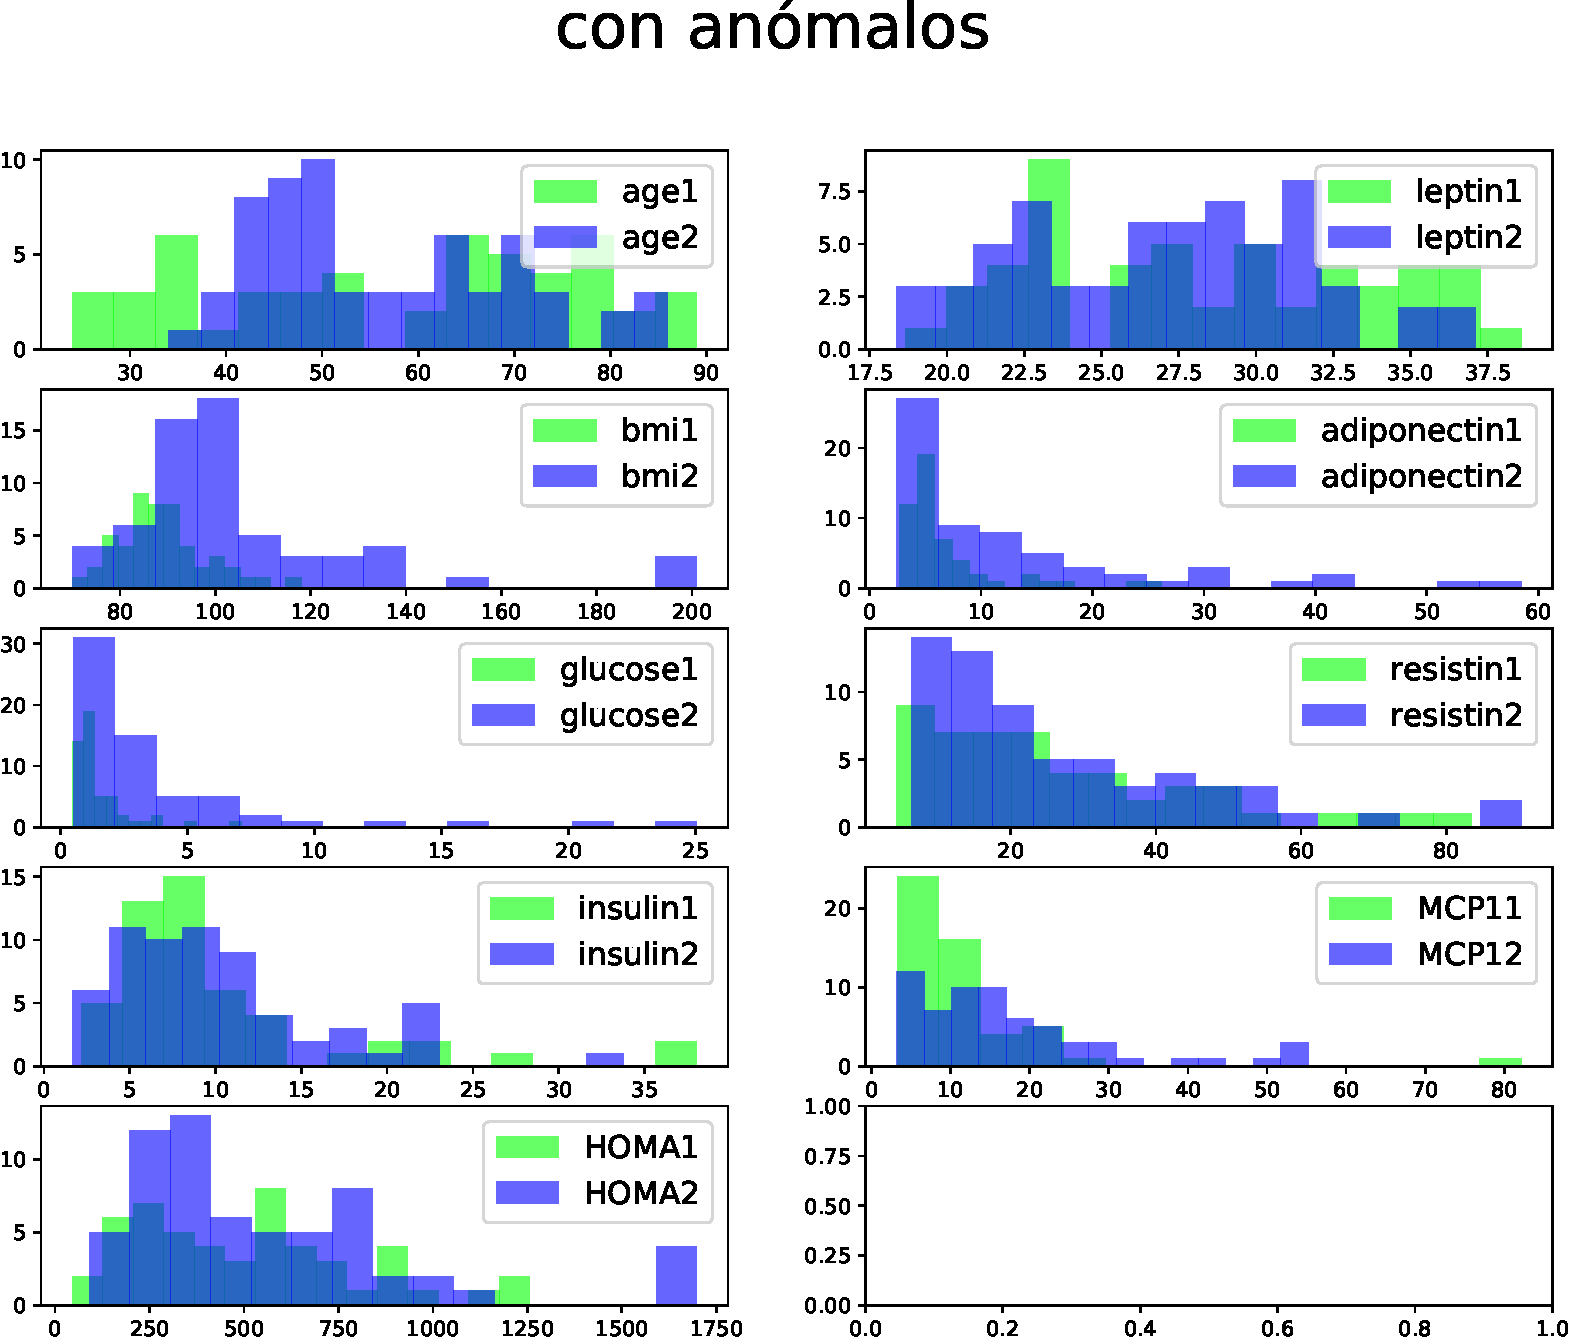
\includegraphics[width = 0.49\linewidth]{../python/images/hist.pdf}
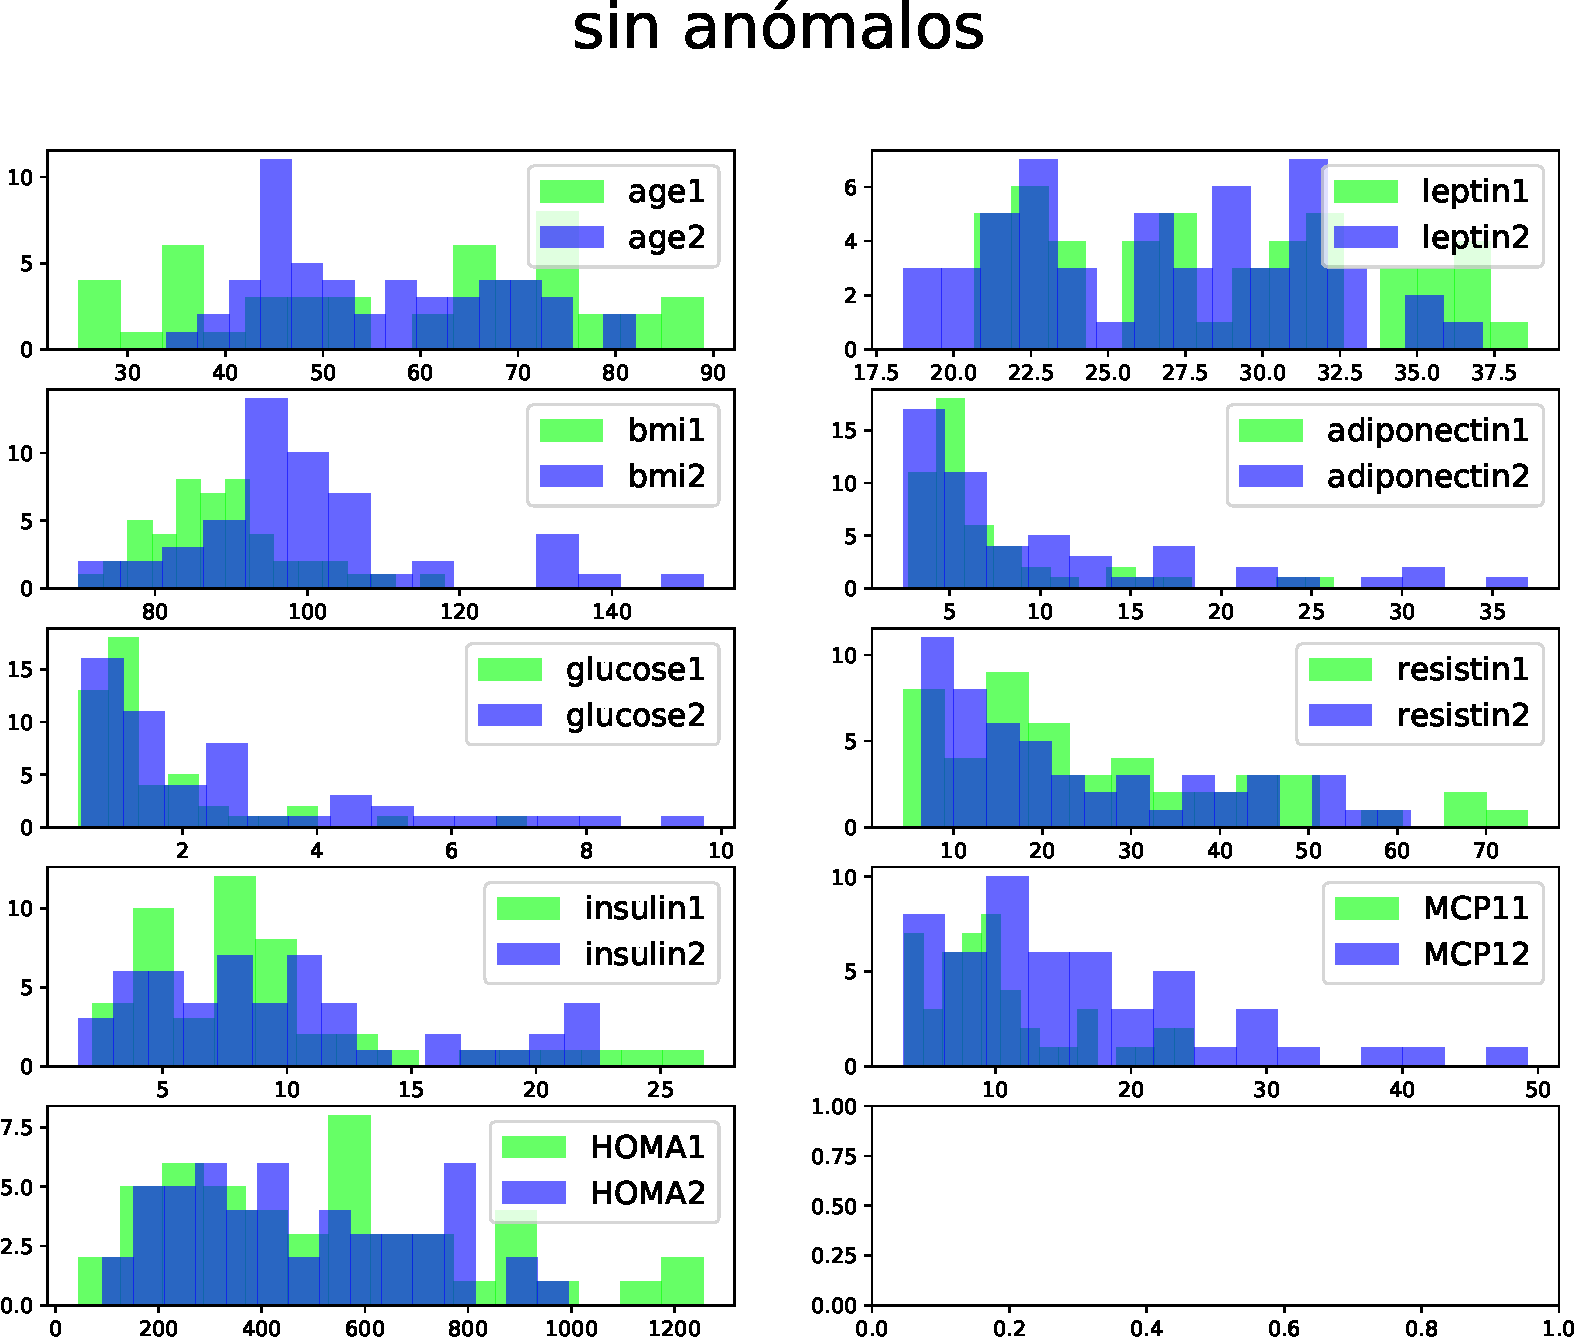
\includegraphics[width = 0.49\linewidth]{../python/images/hist1.pdf}
\figcaption{Histogramas Python para datos con y sin anomalias.}
\label{fig:histsP}
\end{figure}

\lstinputlisting[
	linerange = {9-30},
	caption = {[C\'odigo Python generador de los histogramas con datos an\'omalos.]
	\lstcaption{C\'odigo Python generador de los histogramas con datos an\'omalos.}},
	]{../python/src/histograms.py}

\newpage
\begin{figure}[h]
\centering
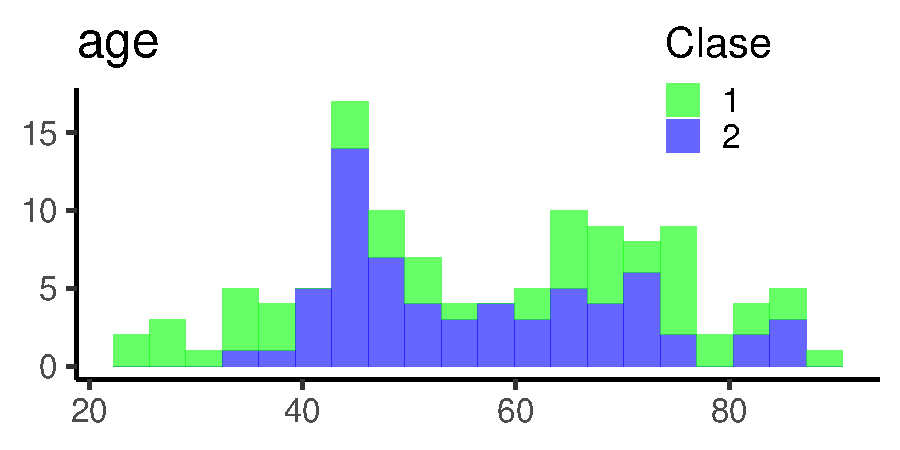
\includegraphics[width = 0.4\linewidth]{../R/images/hist1.pdf}
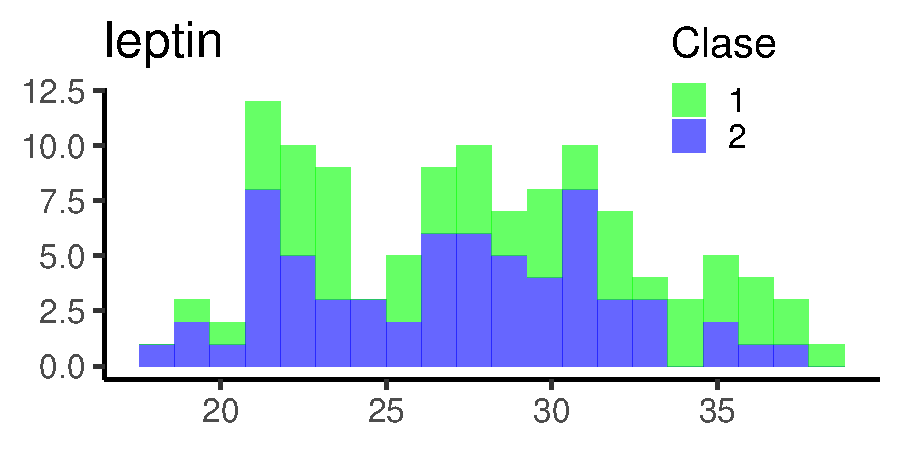
\includegraphics[width = 0.4\linewidth]{../R/images/hist2.pdf}
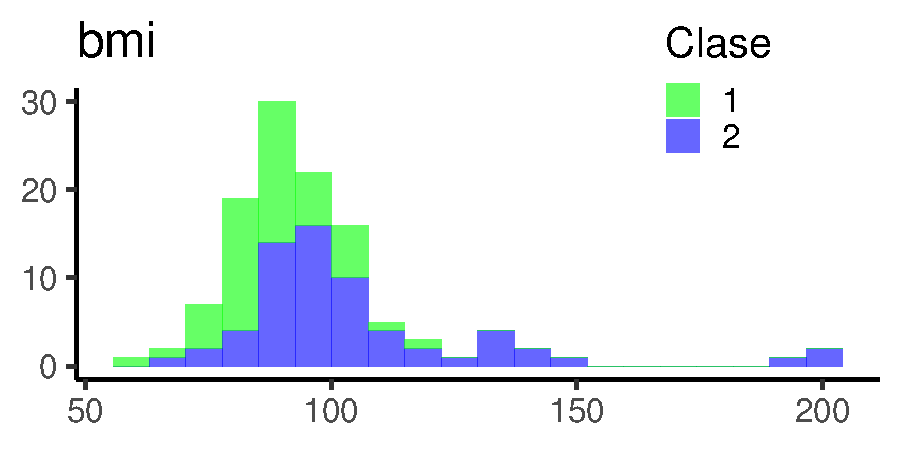
\includegraphics[width = 0.4\linewidth]{../R/images/hist3.pdf}
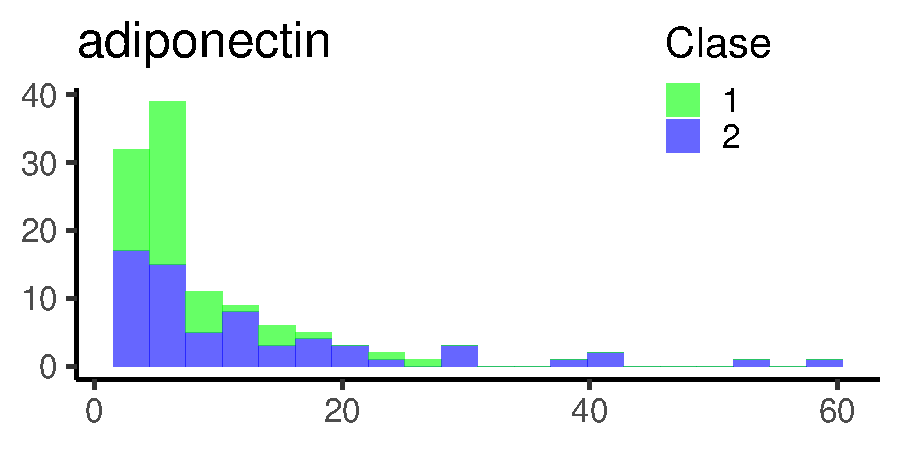
\includegraphics[width = 0.4\linewidth]{../R/images/hist4.pdf}
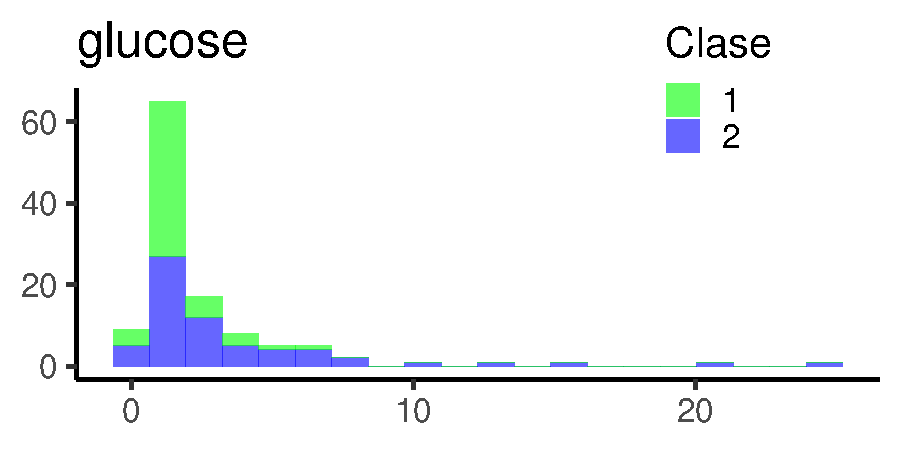
\includegraphics[width = 0.4\linewidth]{../R/images/hist5.pdf}
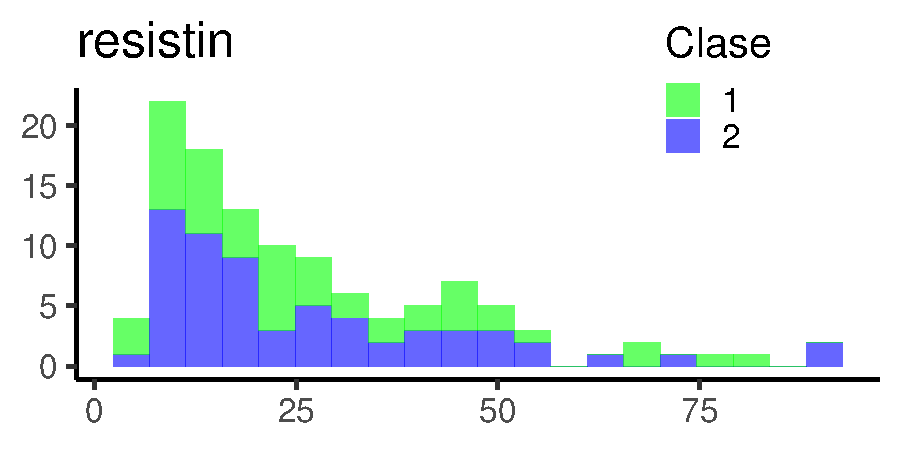
\includegraphics[width = 0.4\linewidth]{../R/images/hist6.pdf}
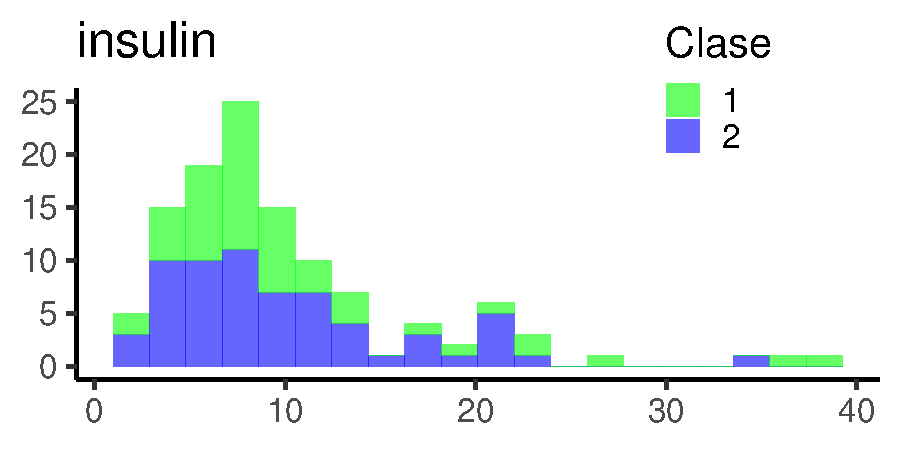
\includegraphics[width = 0.4\linewidth]{../R/images/hist7.pdf}
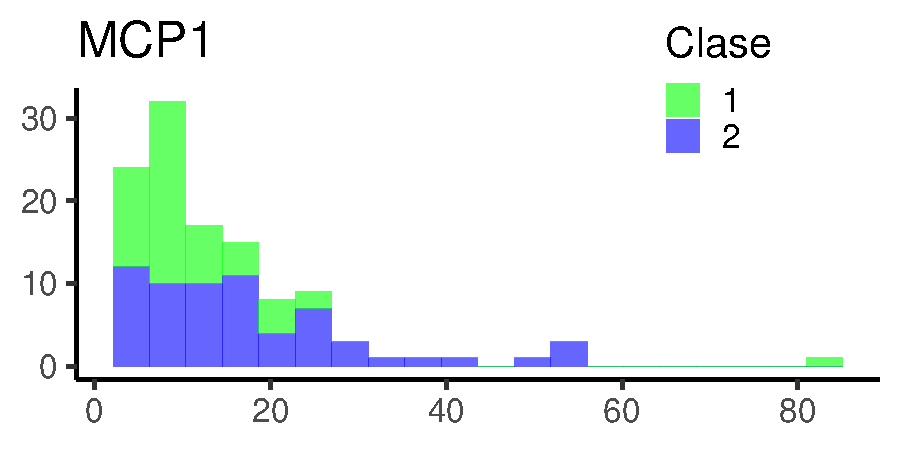
\includegraphics[width = 0.4\linewidth]{../R/images/hist8.pdf}
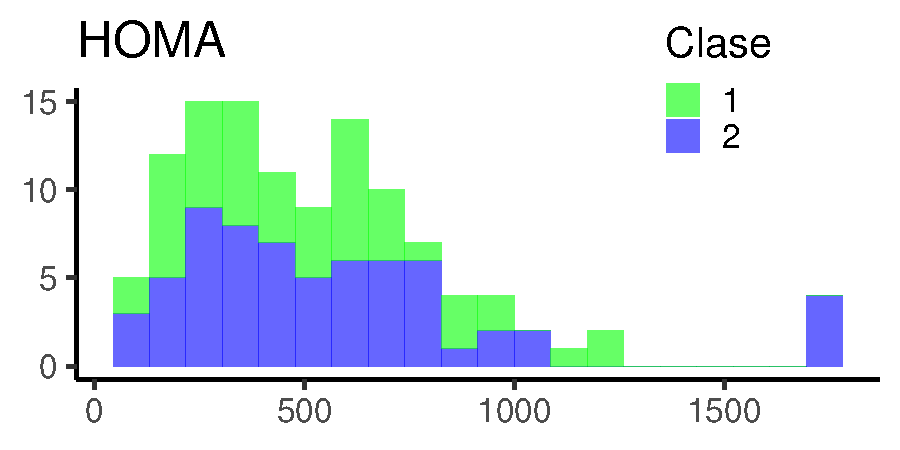
\includegraphics[width = 0.4\linewidth]{../R/images/hist9.pdf}
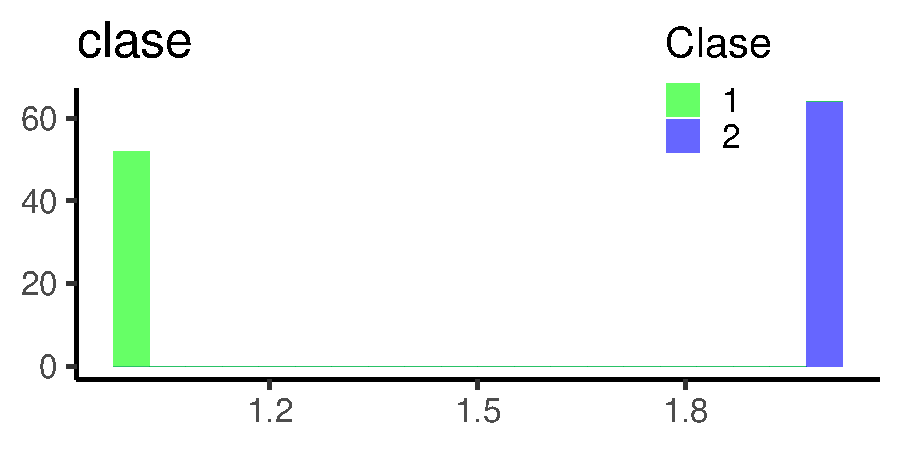
\includegraphics[width = 0.4\linewidth]{../R/images/hist10.pdf}
\figcaption{Histogramas R para datos con anomalias.}
\label{fig:histsR}
\end{figure}

\lstinputlisting[
	linerange = {8-18},
	caption = {[C\'odigo R generador de los histrogramas con datos an\'omalos.]
	\lstcaption{C\'odigo R generador de los histrogramas con datos an\'omalos.}},
	]{../R/src/histograms.r}

\newpage

\begin{figure}[h]
\centering
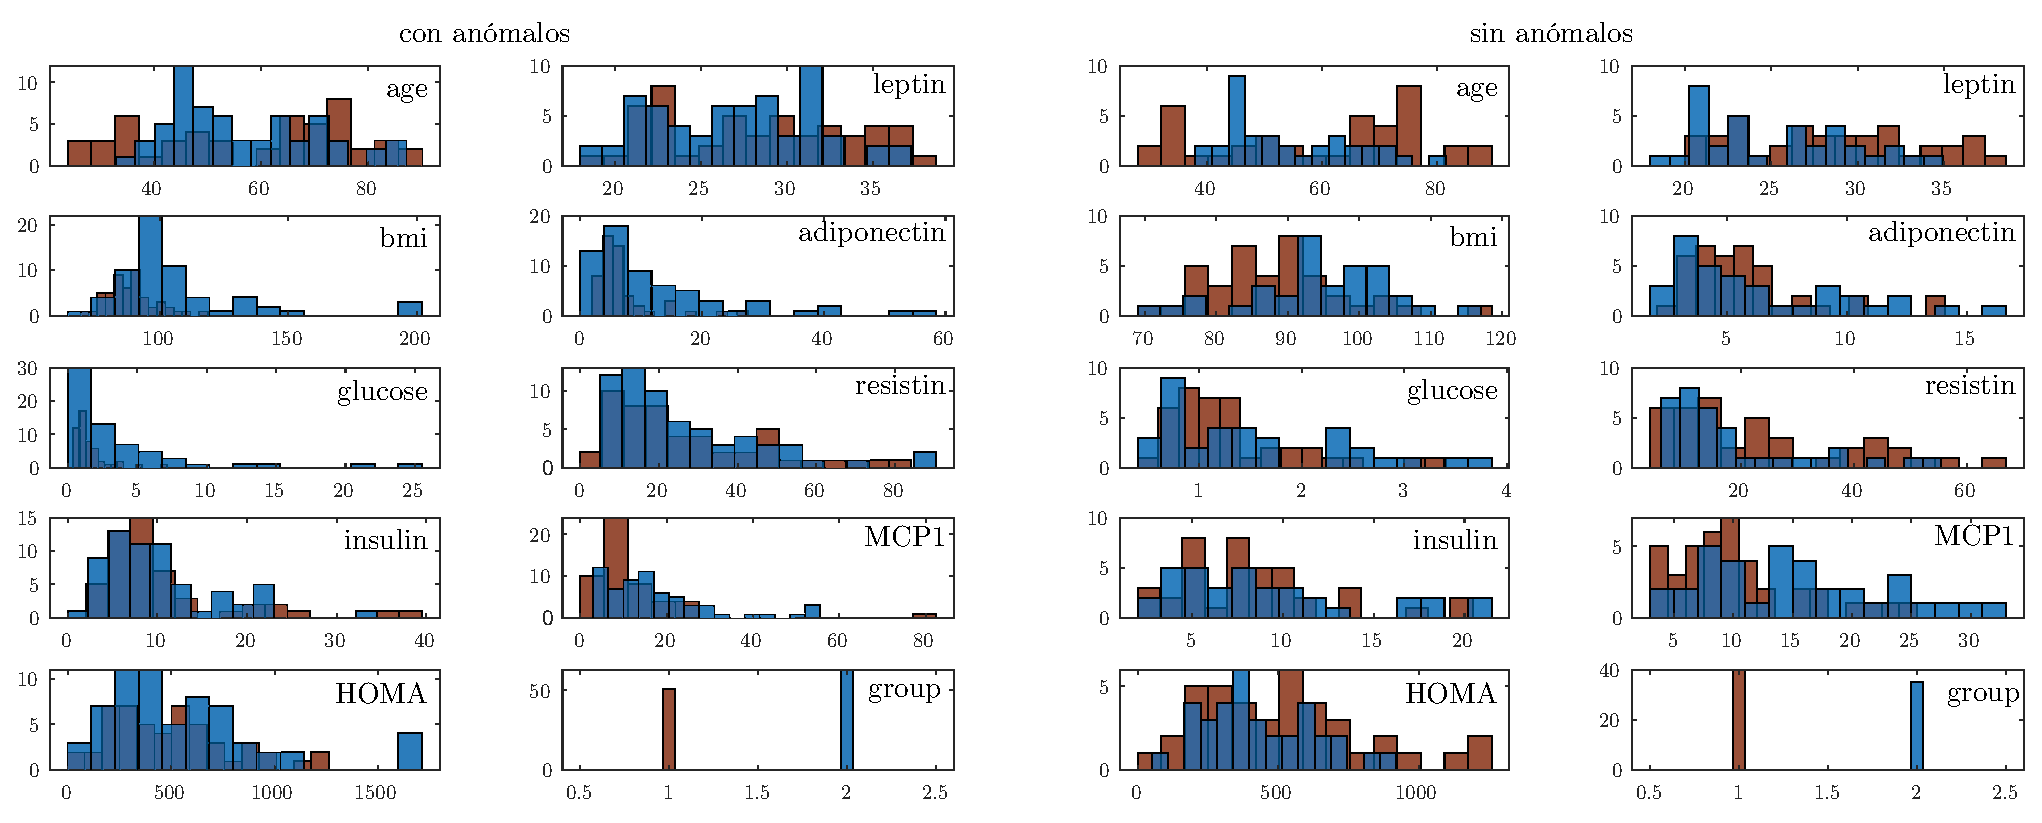
\includegraphics[width = \linewidth]{../matlab/images/hist.eps}
\figcaption{Histogramas Matlab.}
\label{fig:histmatl}
\end{figure}

\begin{lstlisting}[
	style=Matlab-editor,
	frame=single,
	numbers=left,
	label=lst:cod2,
	caption = {[C\'odigo Matlab generador de los histogramas.]
	\lstcaption{C\'odigo Matlab generador de los histogramas.}},
	captionpos=b,
	]
for (i = 1 : 10)
	subplot (5, 2, i);
	histogram (dataR2mat (dataR2mat (:, end) == 1, i), 15);
	hold on;
	histogram (dataR2mat (dataR2mat (:, end) == 2, i), 15);
end
\end{lstlisting}

\newpage

\subsubseccion{Kernel Density}

\begin{figure}[h]
\centering
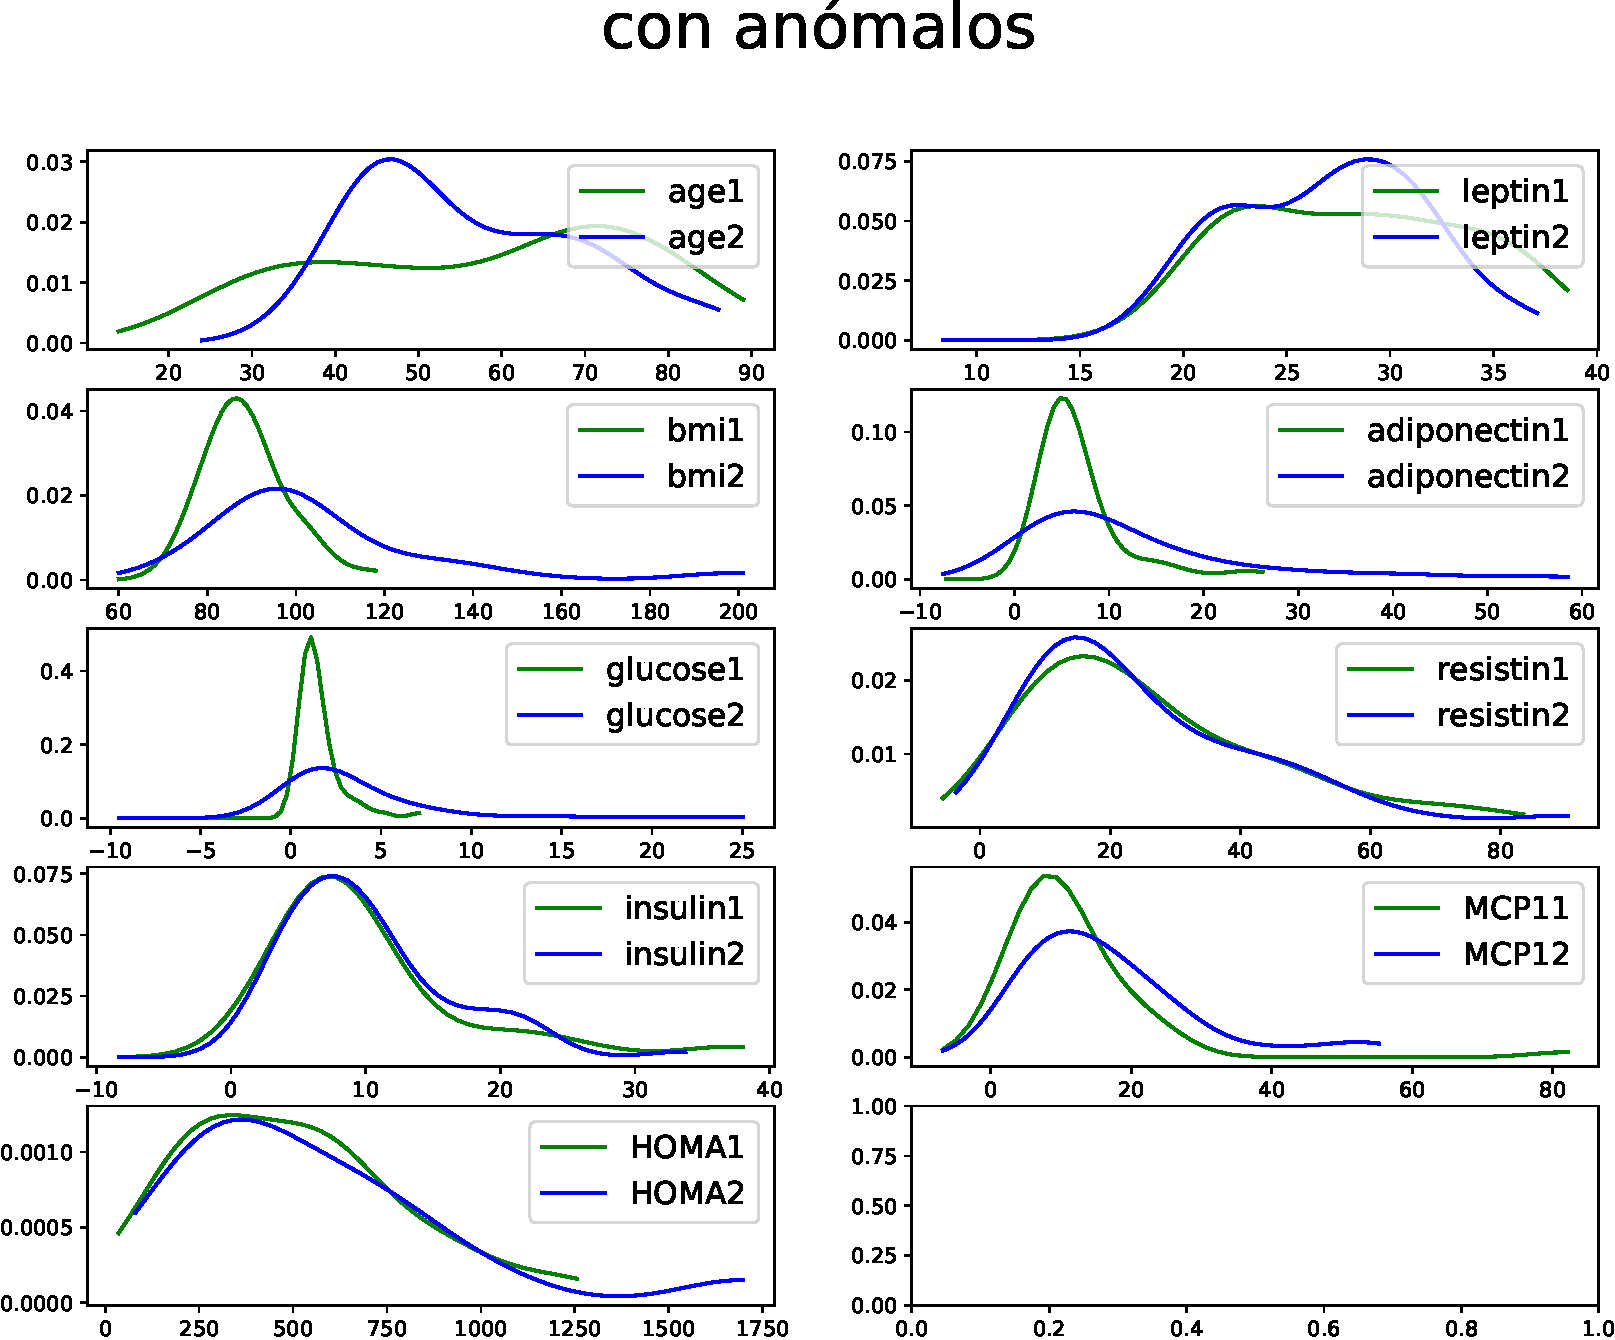
\includegraphics[width = 0.49\linewidth]{../python/images/kden.pdf}
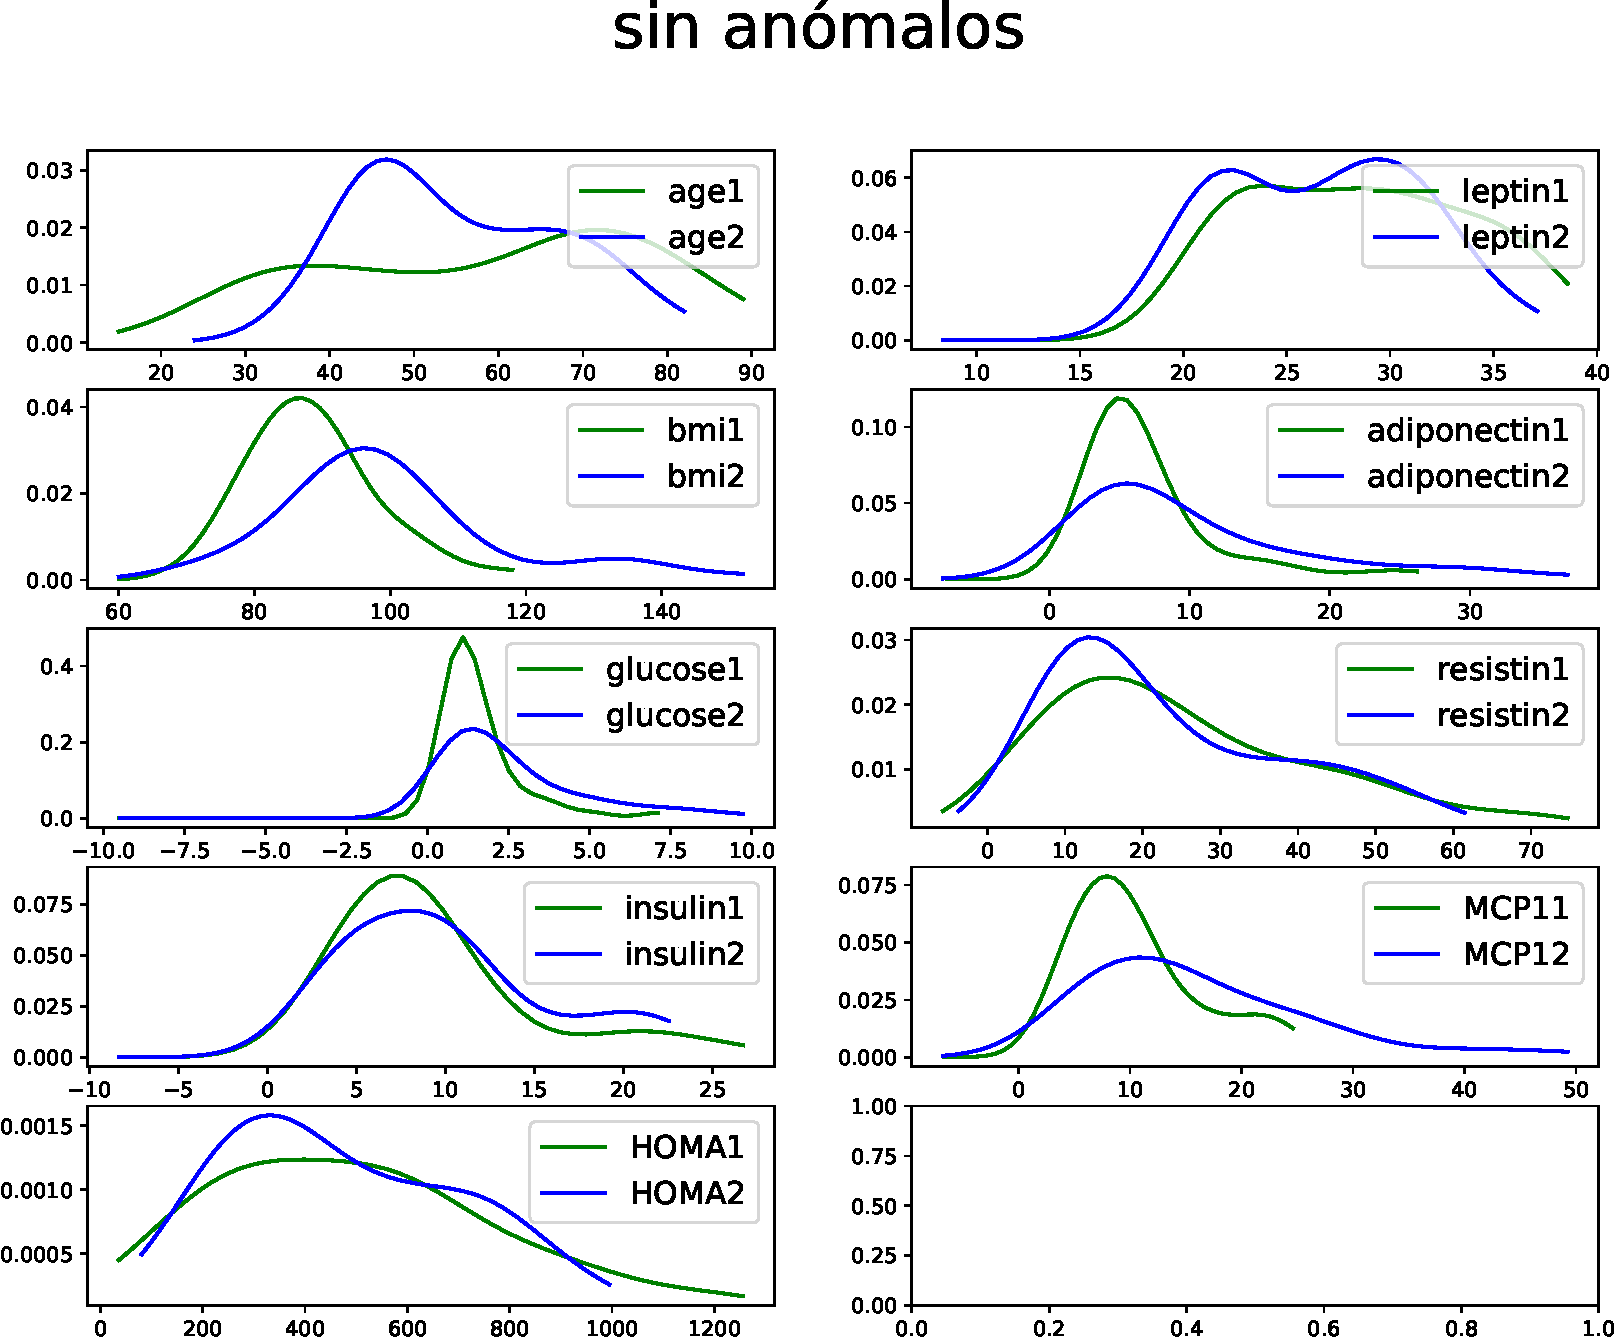
\includegraphics[width = 0.49\linewidth]{../python/images/kden1.pdf}
\figcaption{Kernel Density para datos con y sin anomalias.}
\label{fig:kdens}
\end{figure}

\lstinputlisting[
	linerange = {9-32},
	caption = {[C\'odigo Python generador de los kernel density plots con datos an\'omalos.]
	\lstcaption{C\'odigo Python generador de los kernel density plots con datos an\'omalos.}},
	]{../python/src/kerneldensity.py}
\newpage
\begin{figure}[h]
\centering
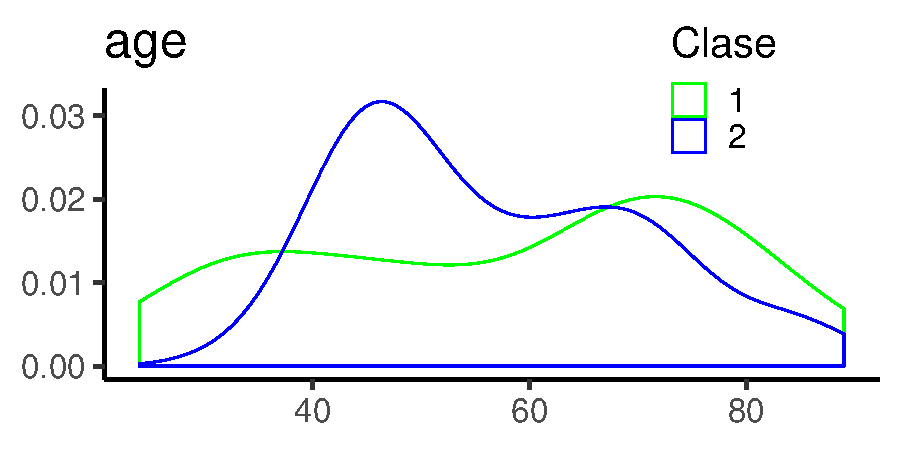
\includegraphics[width = 0.4\linewidth]{../R/images/dens1.pdf}
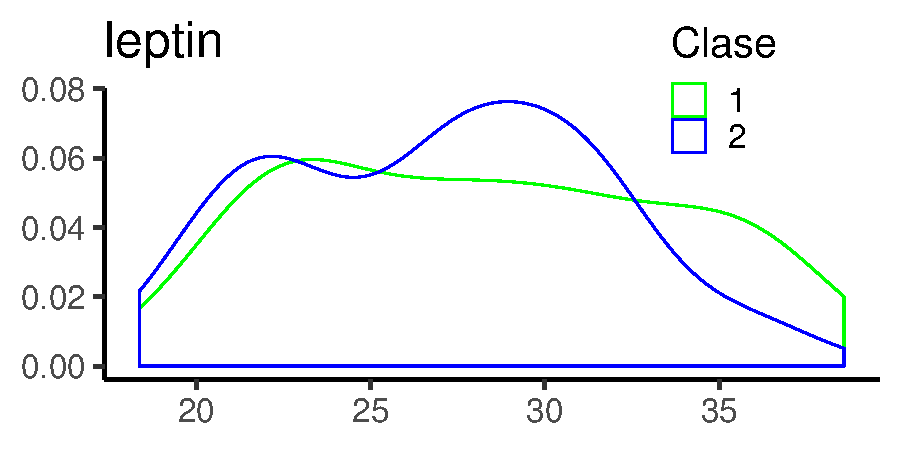
\includegraphics[width = 0.4\linewidth]{../R/images/dens2.pdf}
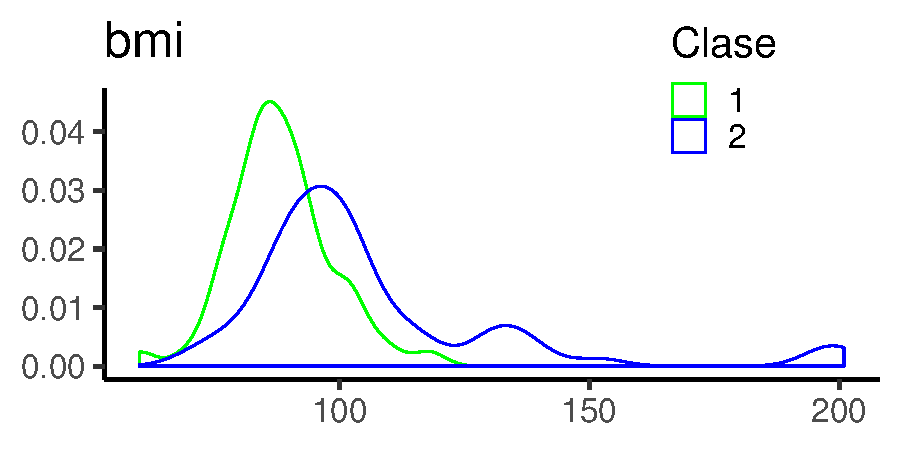
\includegraphics[width = 0.4\linewidth]{../R/images/dens3.pdf}
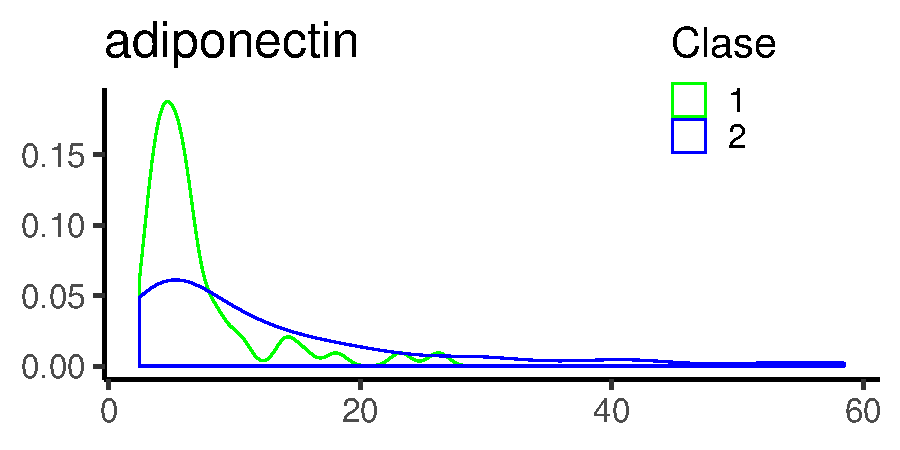
\includegraphics[width = 0.4\linewidth]{../R/images/dens4.pdf}
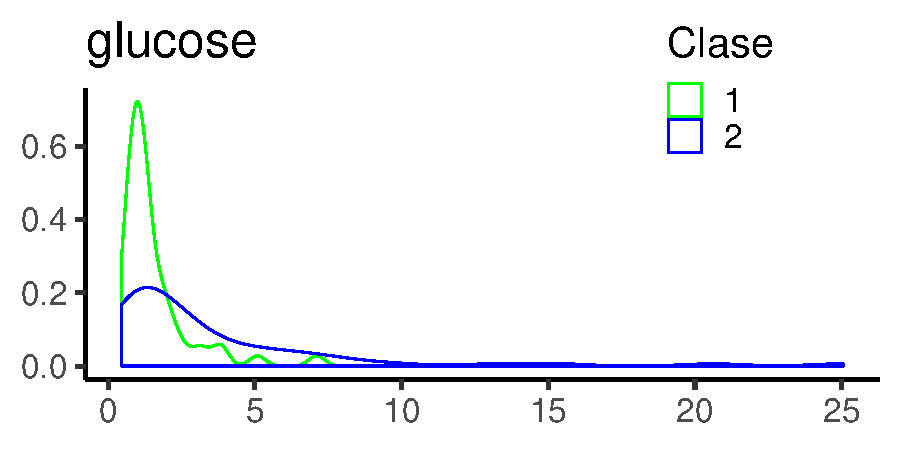
\includegraphics[width = 0.4\linewidth]{../R/images/dens5.pdf}
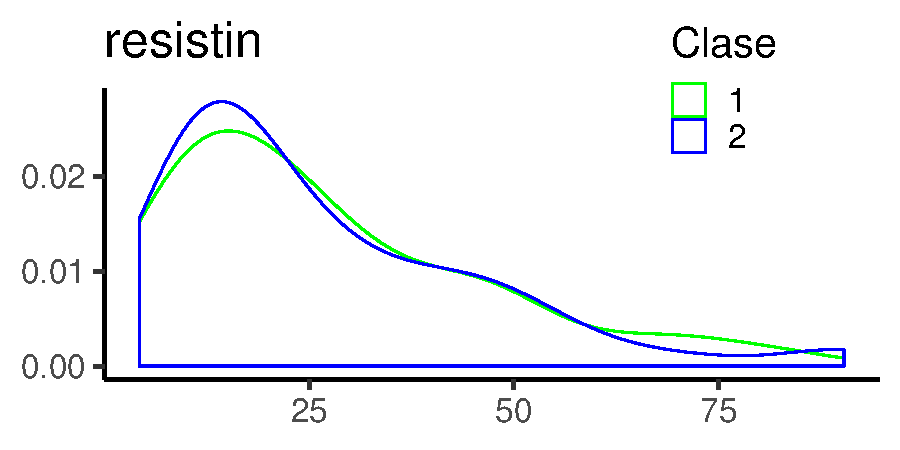
\includegraphics[width = 0.4\linewidth]{../R/images/dens6.pdf}
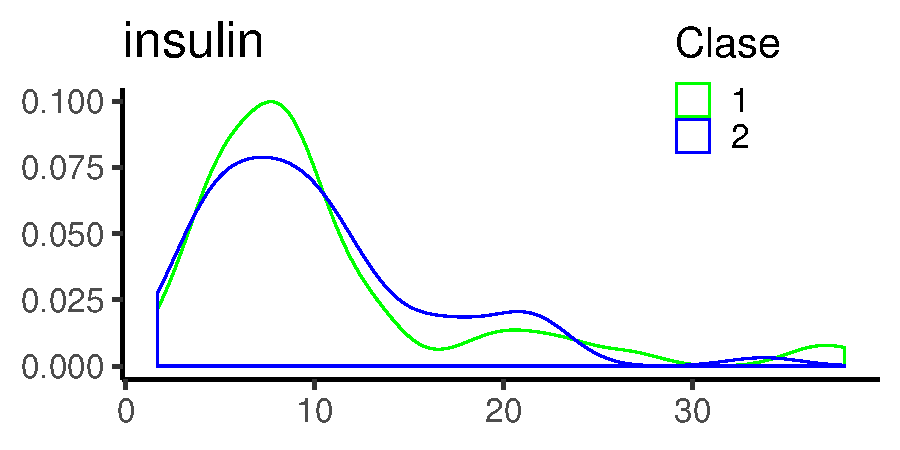
\includegraphics[width = 0.4\linewidth]{../R/images/dens7.pdf}
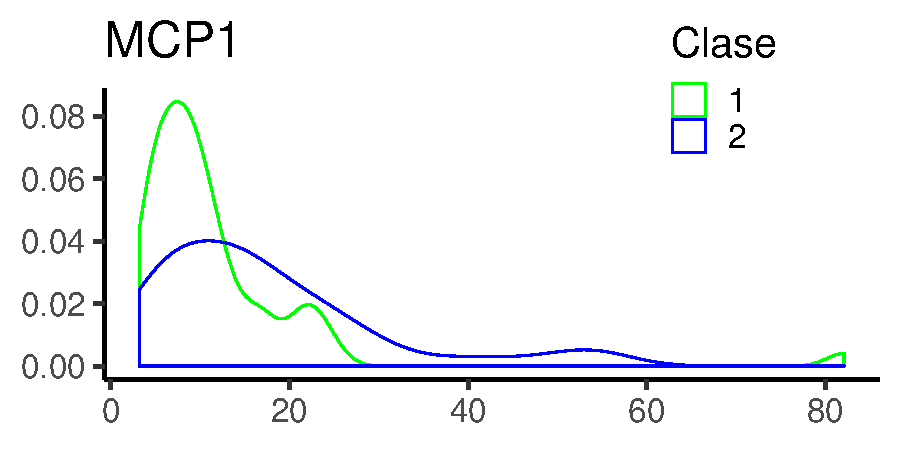
\includegraphics[width = 0.4\linewidth]{../R/images/dens8.pdf}
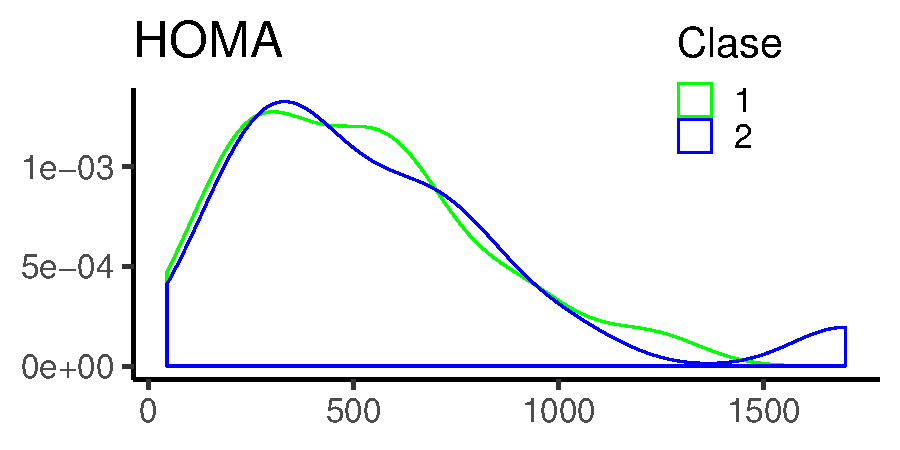
\includegraphics[width = 0.4\linewidth]{../R/images/dens9.pdf}
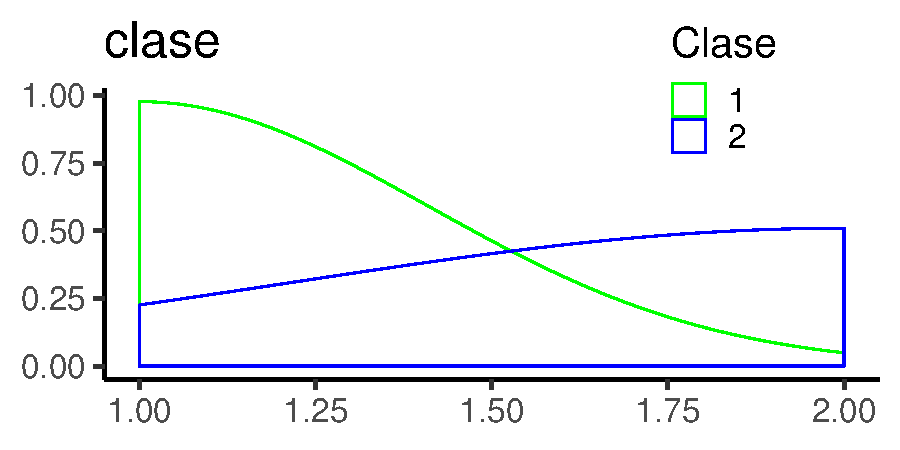
\includegraphics[width = 0.4\linewidth]{../R/images/dens10.pdf}
\figcaption{Gr\'aficos de densidad R.}
\label{fig:densR}
\end{figure}

\lstinputlisting[
	linerange = {8-18},
	caption = {[C\'odigo R generador de los density plots.]
	\lstcaption{C\'odigo R generador de los density plots.}},
	]{../R/src/kerneldensity.r}
\newpage

\begin{figure}[h]
\centering
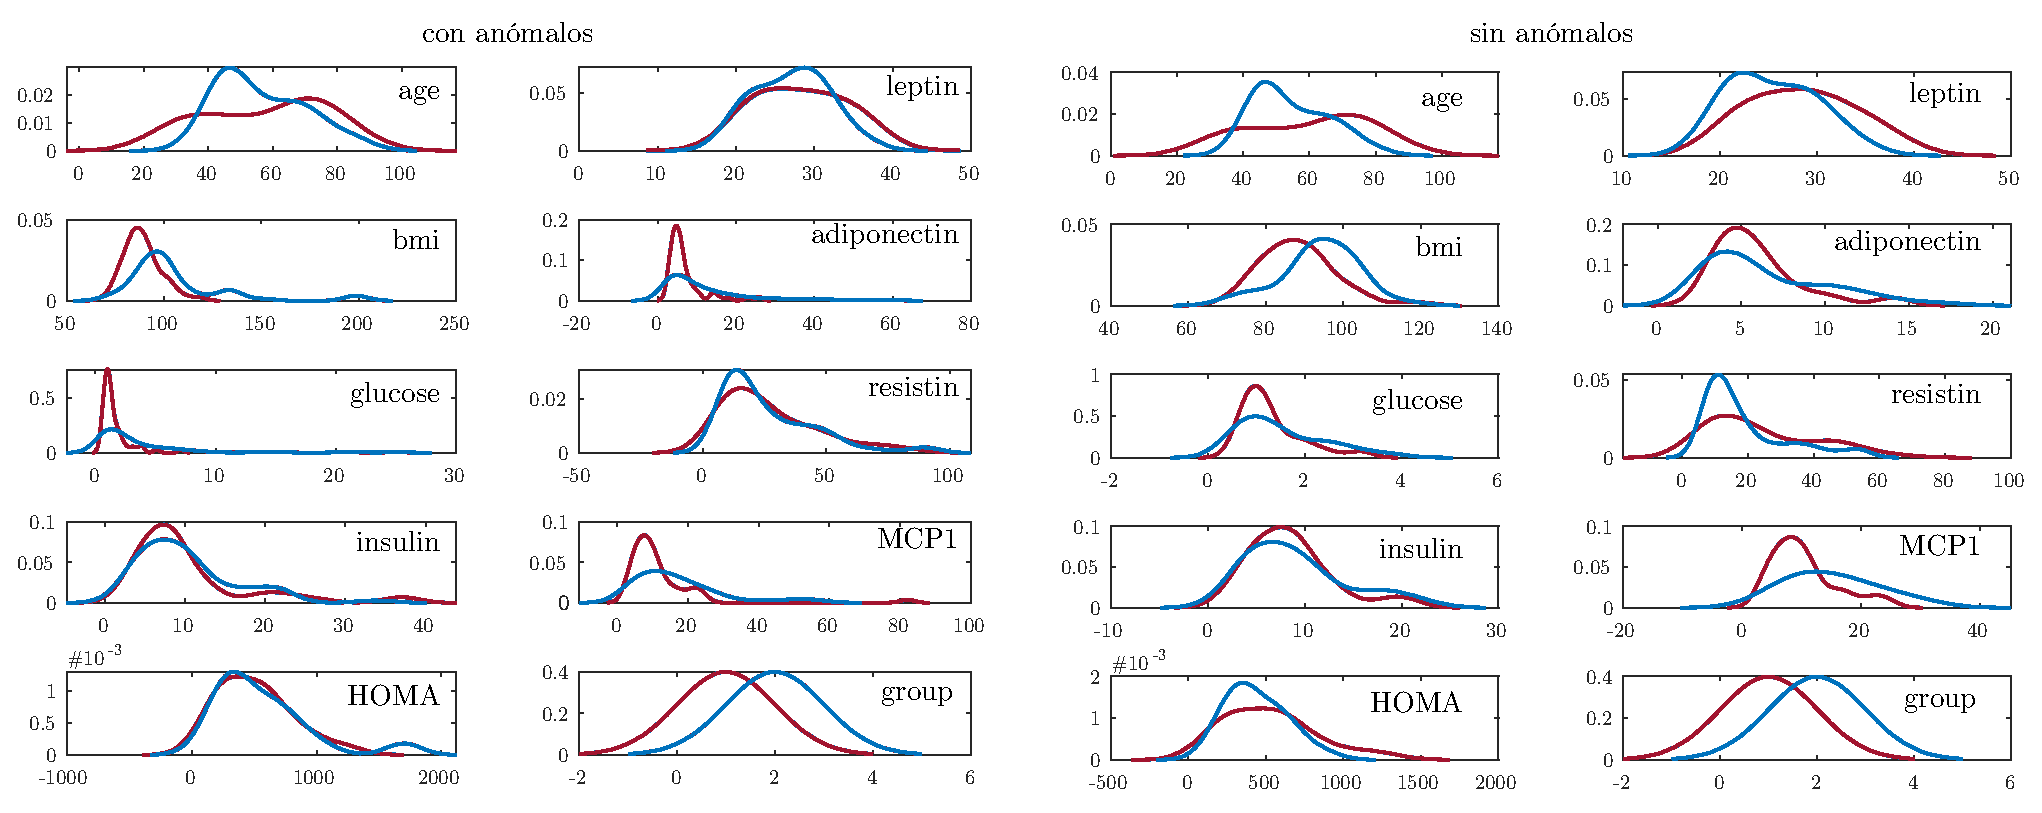
\includegraphics[width = \linewidth]{../matlab/images/ksden.eps}
\figcaption{Gr\'aficos de densidad Matlab.}
\end{figure}

\begin{lstlisting}[
	style=Matlab-editor,
	frame=single,
	numbers=left,
	caption = {[C\'odigo Matlab generador de los kdensity.]
	\lstcaption{C\'odigo Matlab generador de los kdensity.}},
	captionpos=b,
	]
for (i = 1 : 10)
	subplot (5, 2, i);
	ksdensity (dataR2mat (dataR2mat (:, end) == 1, i));
	hold on;
	ksdensity (dataR2mat (dataR2mat (:, end) == 2, i));
end
\end{lstlisting}

\newpage

\subsubseccion{Boxplot}

\begin{figure}[h]
\centering
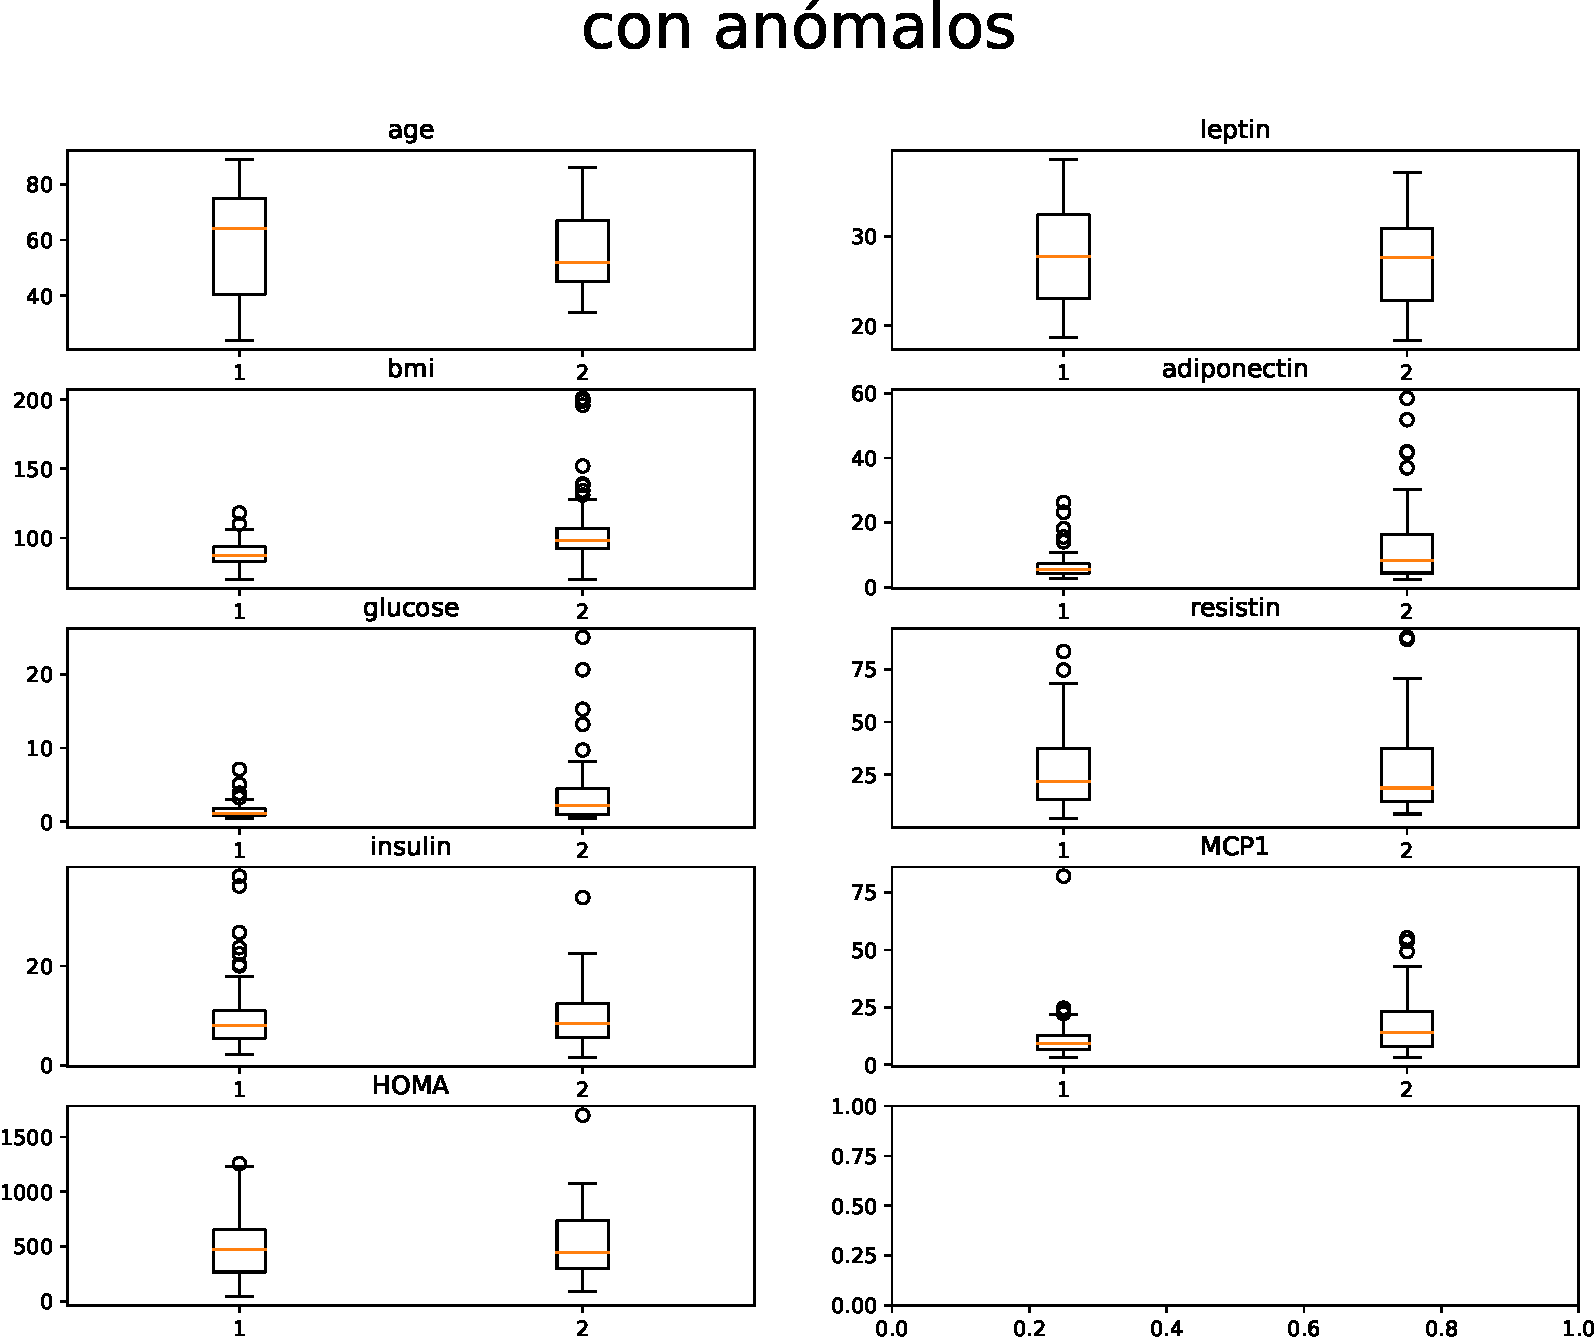
\includegraphics[width = 0.49\linewidth]{../python/images/boxp.pdf}
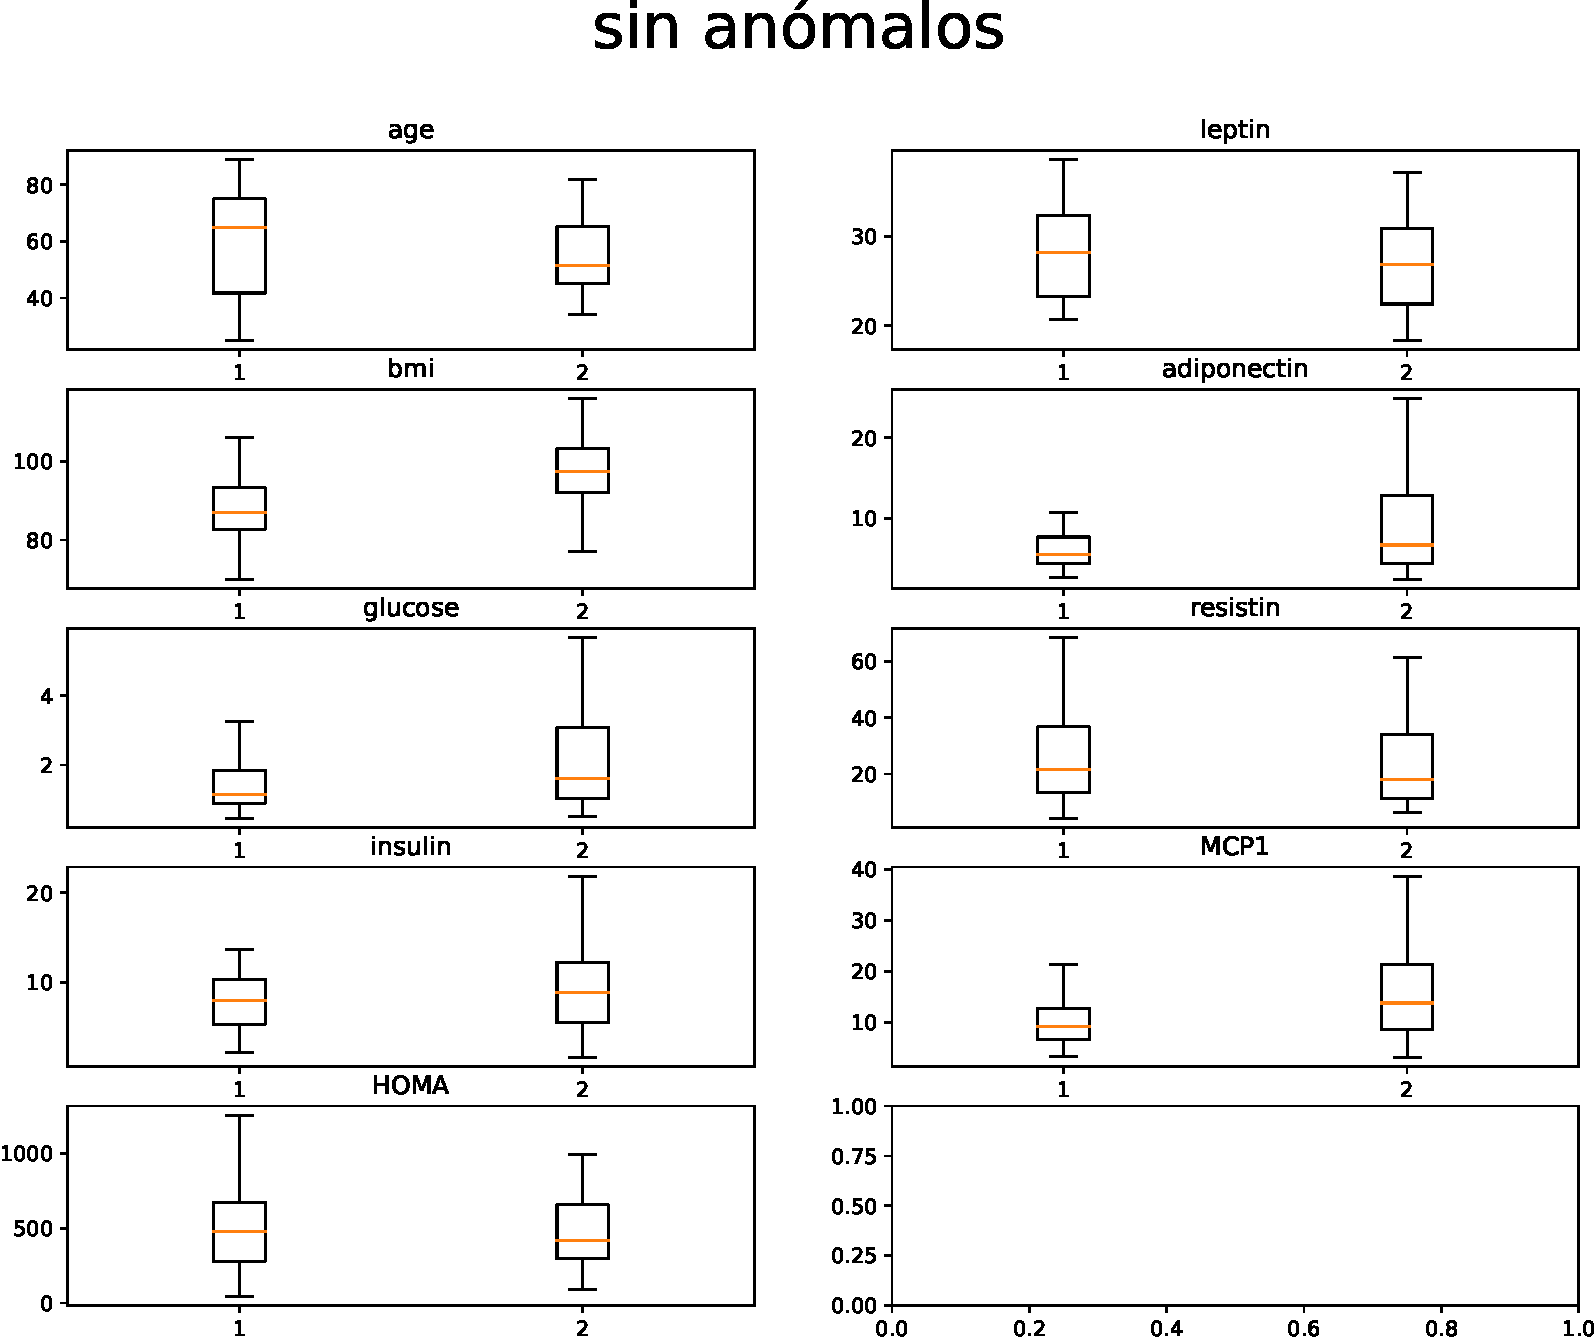
\includegraphics[width = 0.49\linewidth]{../python/images/boxp1.pdf}
\figcaption{Boxplots Python para datos con y sin anomalias.}
\label{fig:boxP}
\end{figure}

\lstinputlisting[
	linerange = {9-24},
	caption = {[C\'odigo Python generador de los boxplots con datos an\'omalos.]
	\lstcaption{C\'odigo Python generador de los boxplots con datos an\'omalos.}},
	]{../python/src/boxplot.py}

\newpage

\begin{figure}[h]
\centering
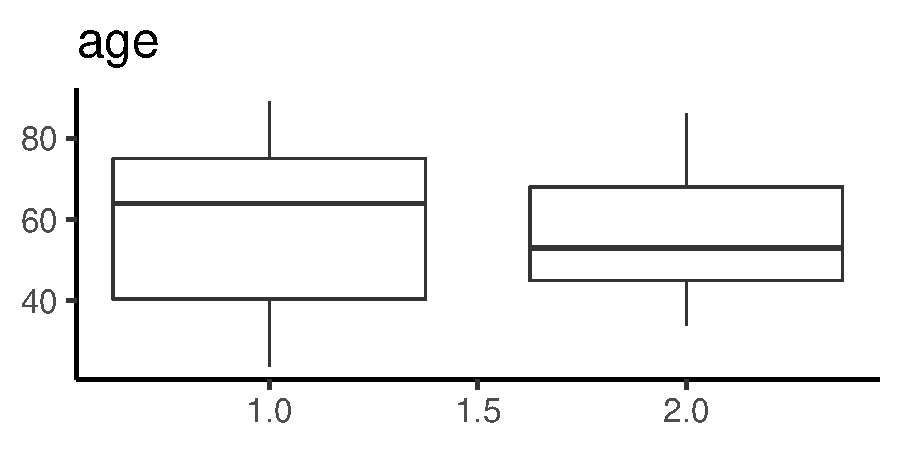
\includegraphics[width = 0.4\linewidth]{../R/images/box1.pdf}
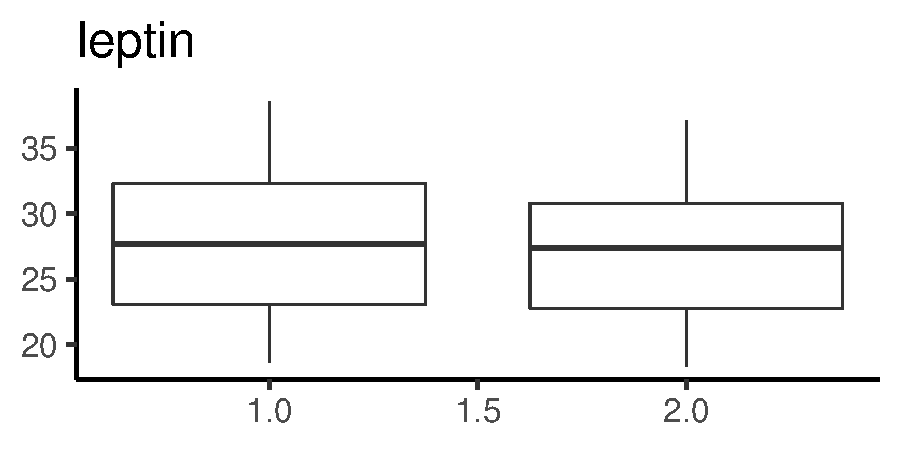
\includegraphics[width = 0.4\linewidth]{../R/images/box2.pdf}
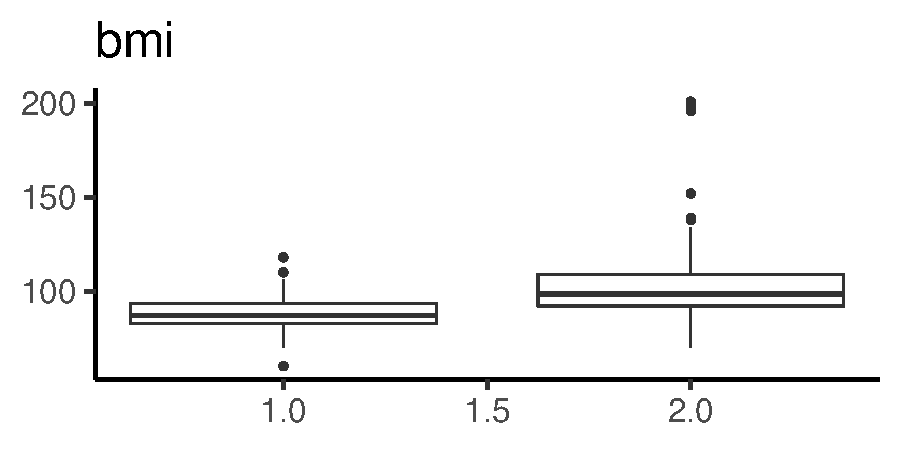
\includegraphics[width = 0.4\linewidth]{../R/images/box3.pdf}
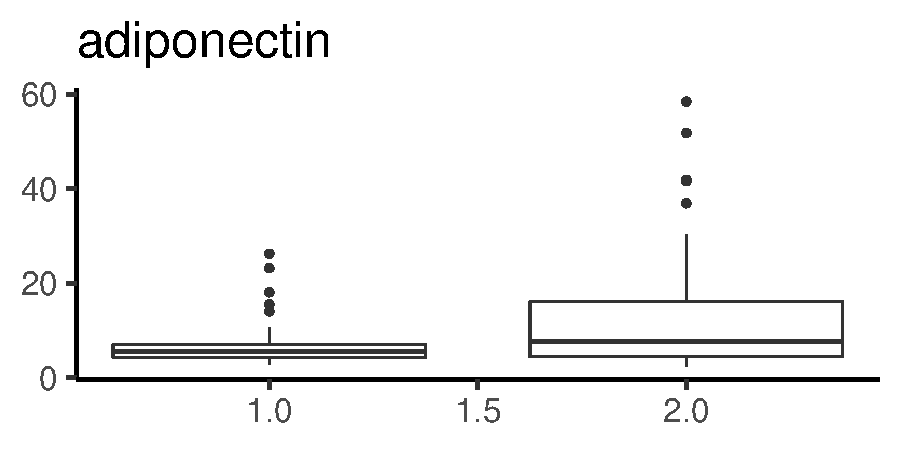
\includegraphics[width = 0.4\linewidth]{../R/images/box4.pdf}
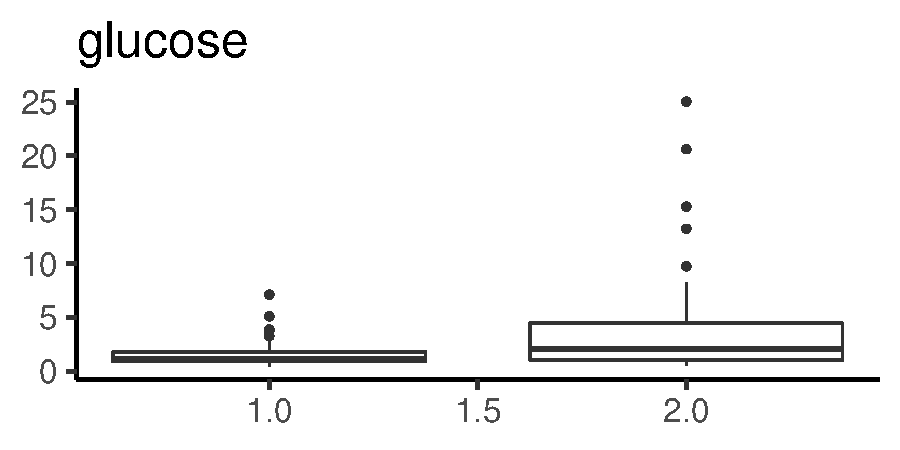
\includegraphics[width = 0.4\linewidth]{../R/images/box5.pdf}
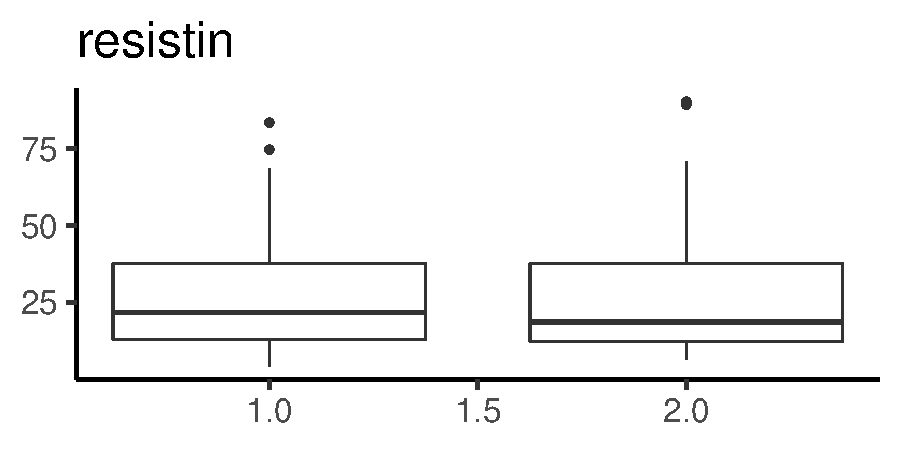
\includegraphics[width = 0.4\linewidth]{../R/images/box6.pdf}
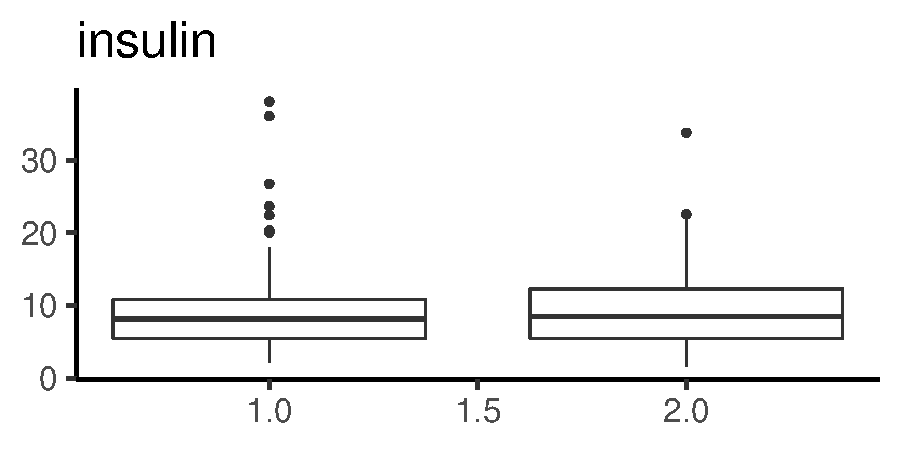
\includegraphics[width = 0.4\linewidth]{../R/images/box7.pdf}
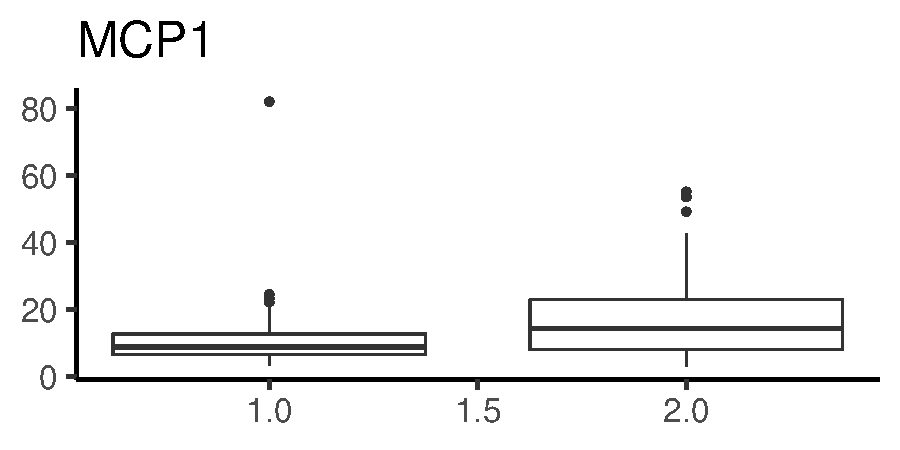
\includegraphics[width = 0.4\linewidth]{../R/images/box8.pdf}
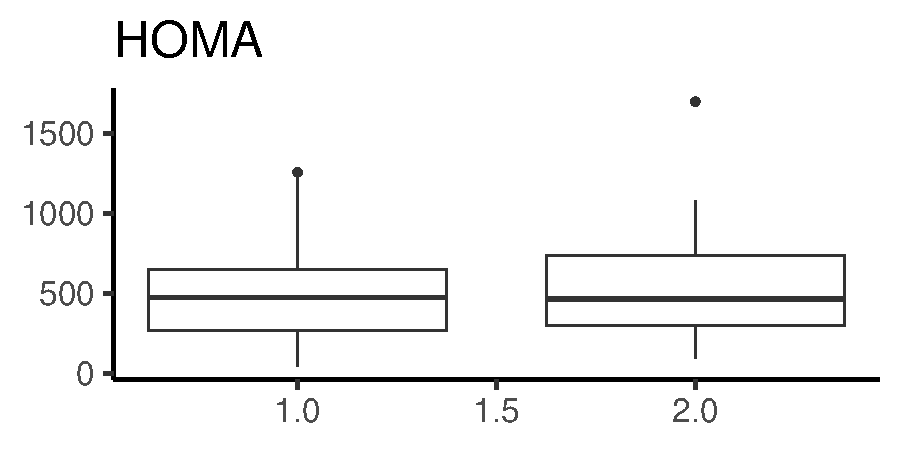
\includegraphics[width = 0.4\linewidth]{../R/images/box9.pdf}
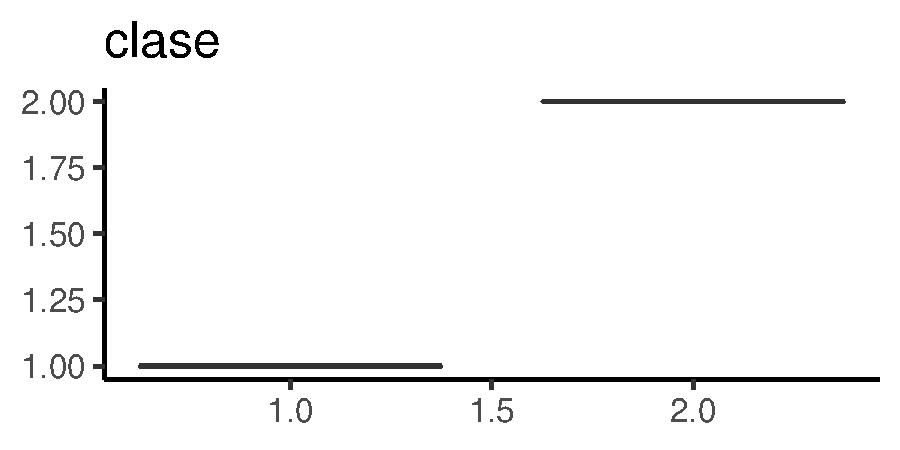
\includegraphics[width = 0.4\linewidth]{../R/images/box10.pdf}
\figcaption{Boxplots R para datos con anomalias.}
\label{fig:boxR}
\end{figure}

\lstinputlisting[
	linerange = {8-18},
	caption = {[C\'odigo R generador de los boxplots.]
	\lstcaption{C\'odigo R generador de los boxplots.}},
	]{../R/src/boxplot.r}

\newpage

\begin{figure}[h]
\centering
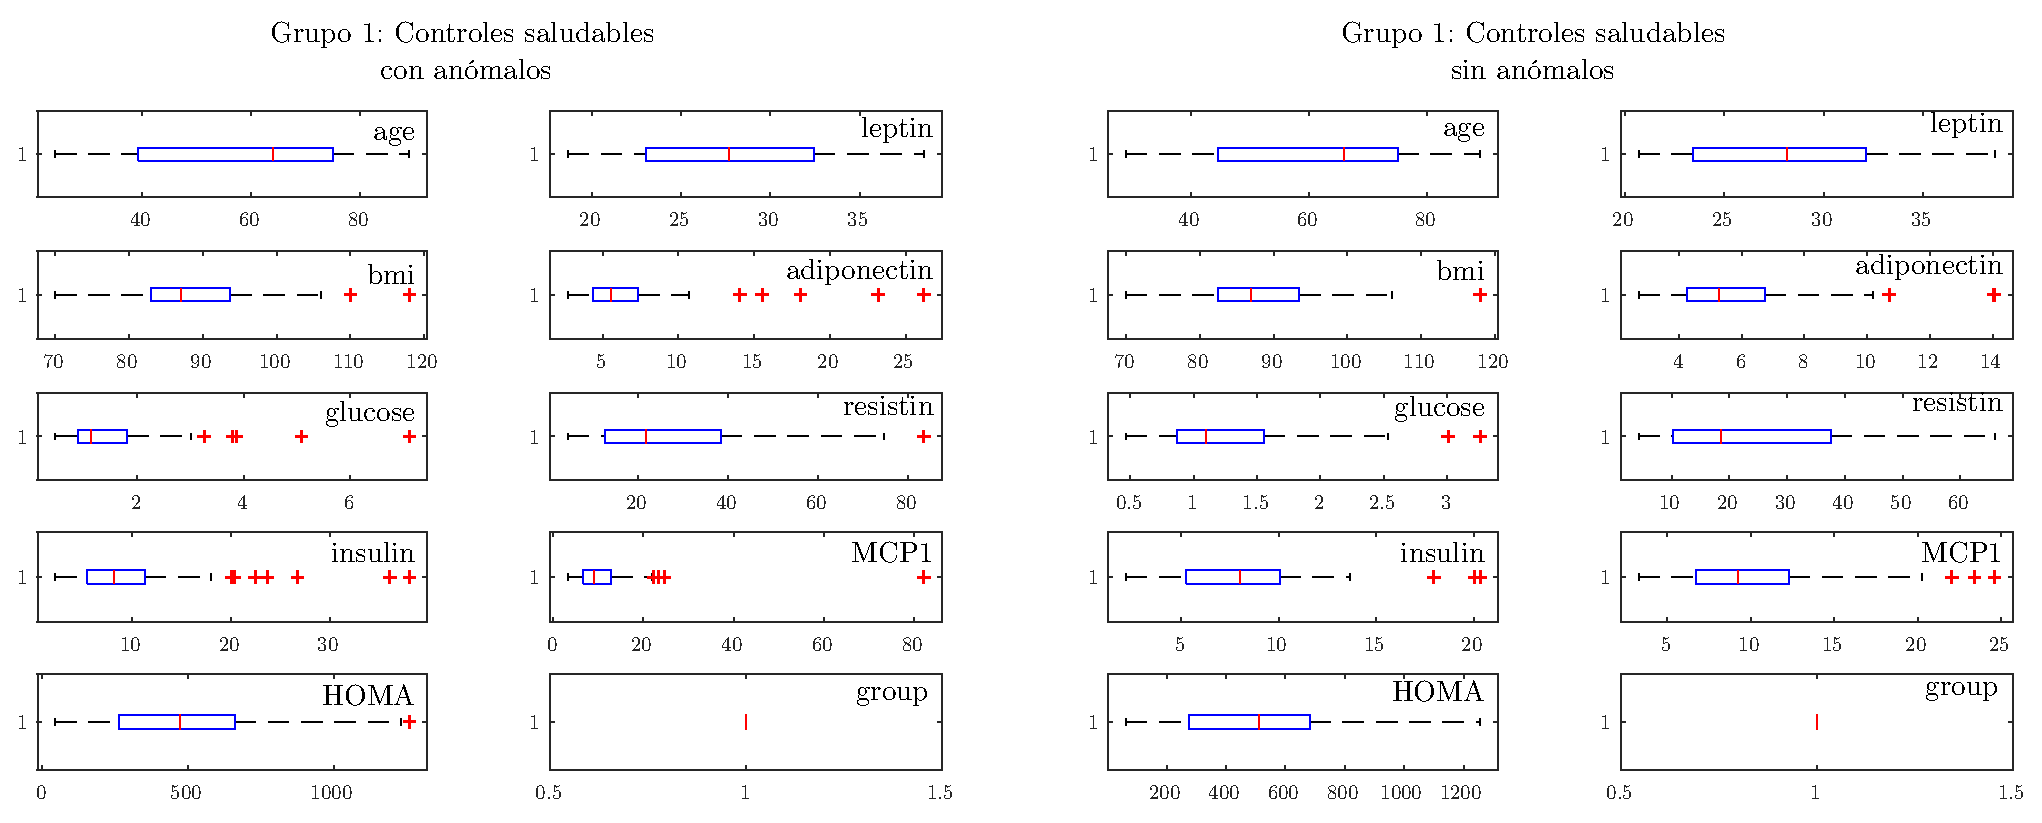
\includegraphics[width = \linewidth]{../matlab/images/box1.eps}
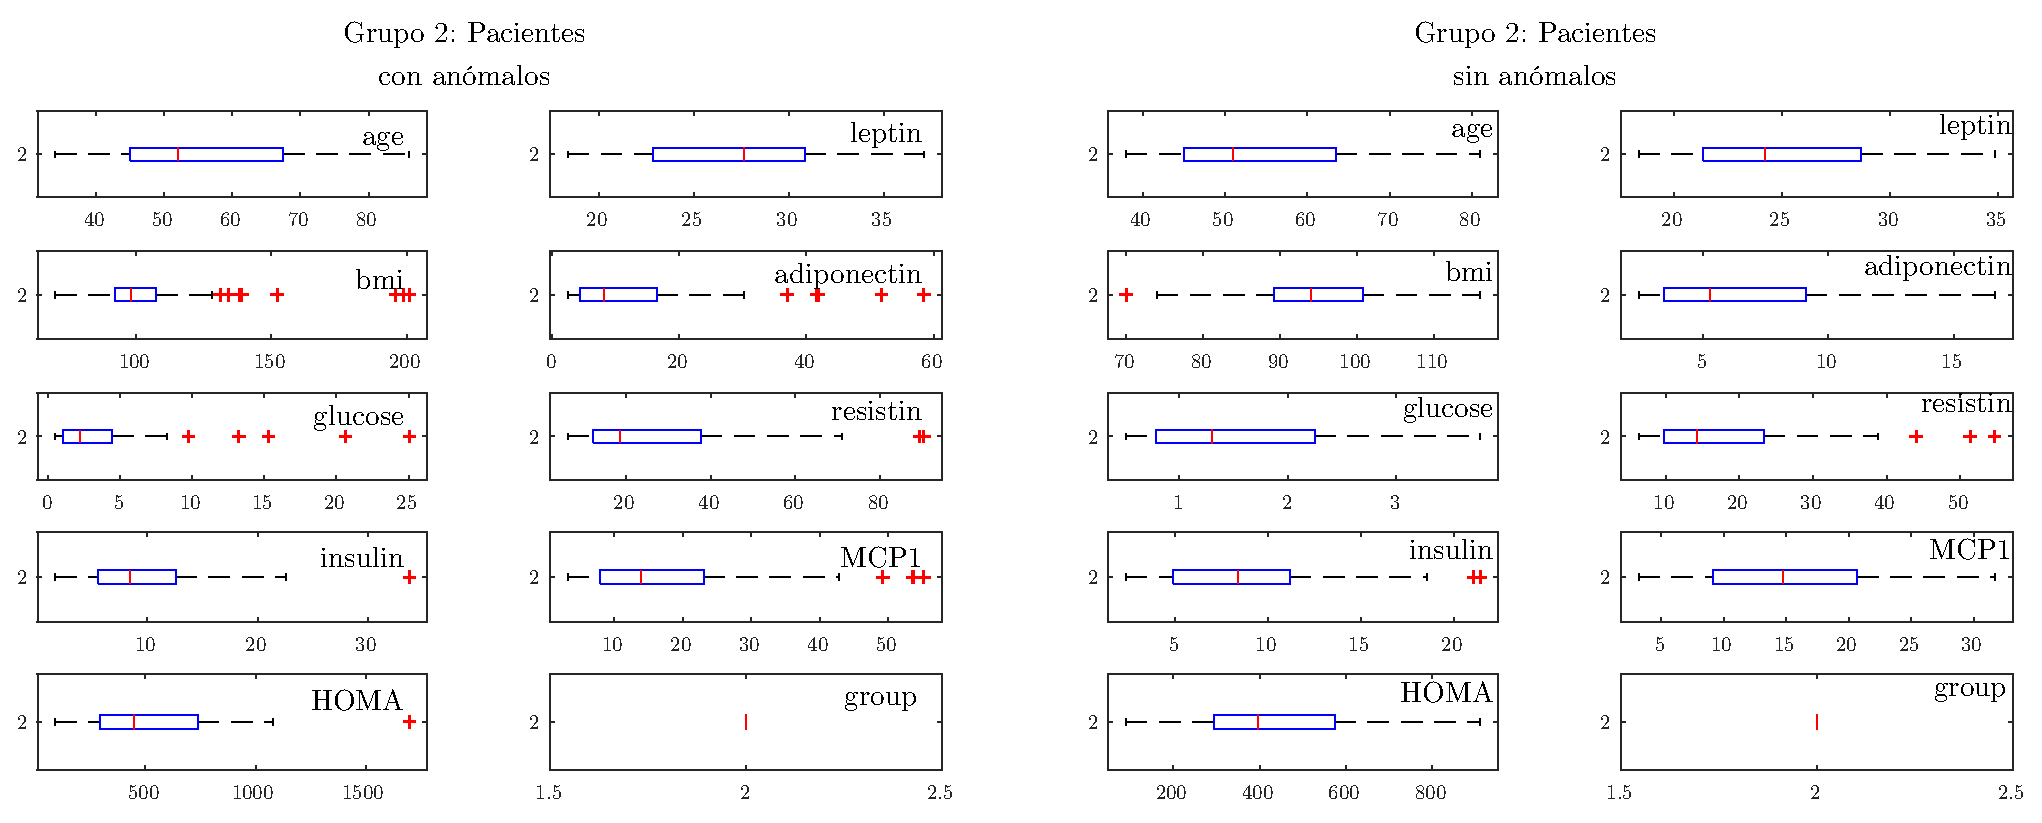
\includegraphics[width = \linewidth]{../matlab/images/box2.eps}
\figcaption{Boxplots Matlab para datos con anomalias.}
\end{figure}

\begin{lstlisting}[
	style=Matlab-editor,
	frame=single,
	numbers=left,
	caption = {[C\'odigo Matlab generador de los boxplots.]
	\lstcaption{C\'odigo Matlab generador de los boxplots.}},
	captionpos=b,
	]
for (i = 1 : 10)
	subplot (5, 2, i);
	boxplot (dataR2mat (dataR2mat (:, end) == 1, i));
	hold on;
	boxplot (dataR2mat (dataR2mat (:, end) == 2, i));
end
\end{lstlisting}
\newpage
\subsubseccion{QQplot}

\begin{figure}[h]
\centering
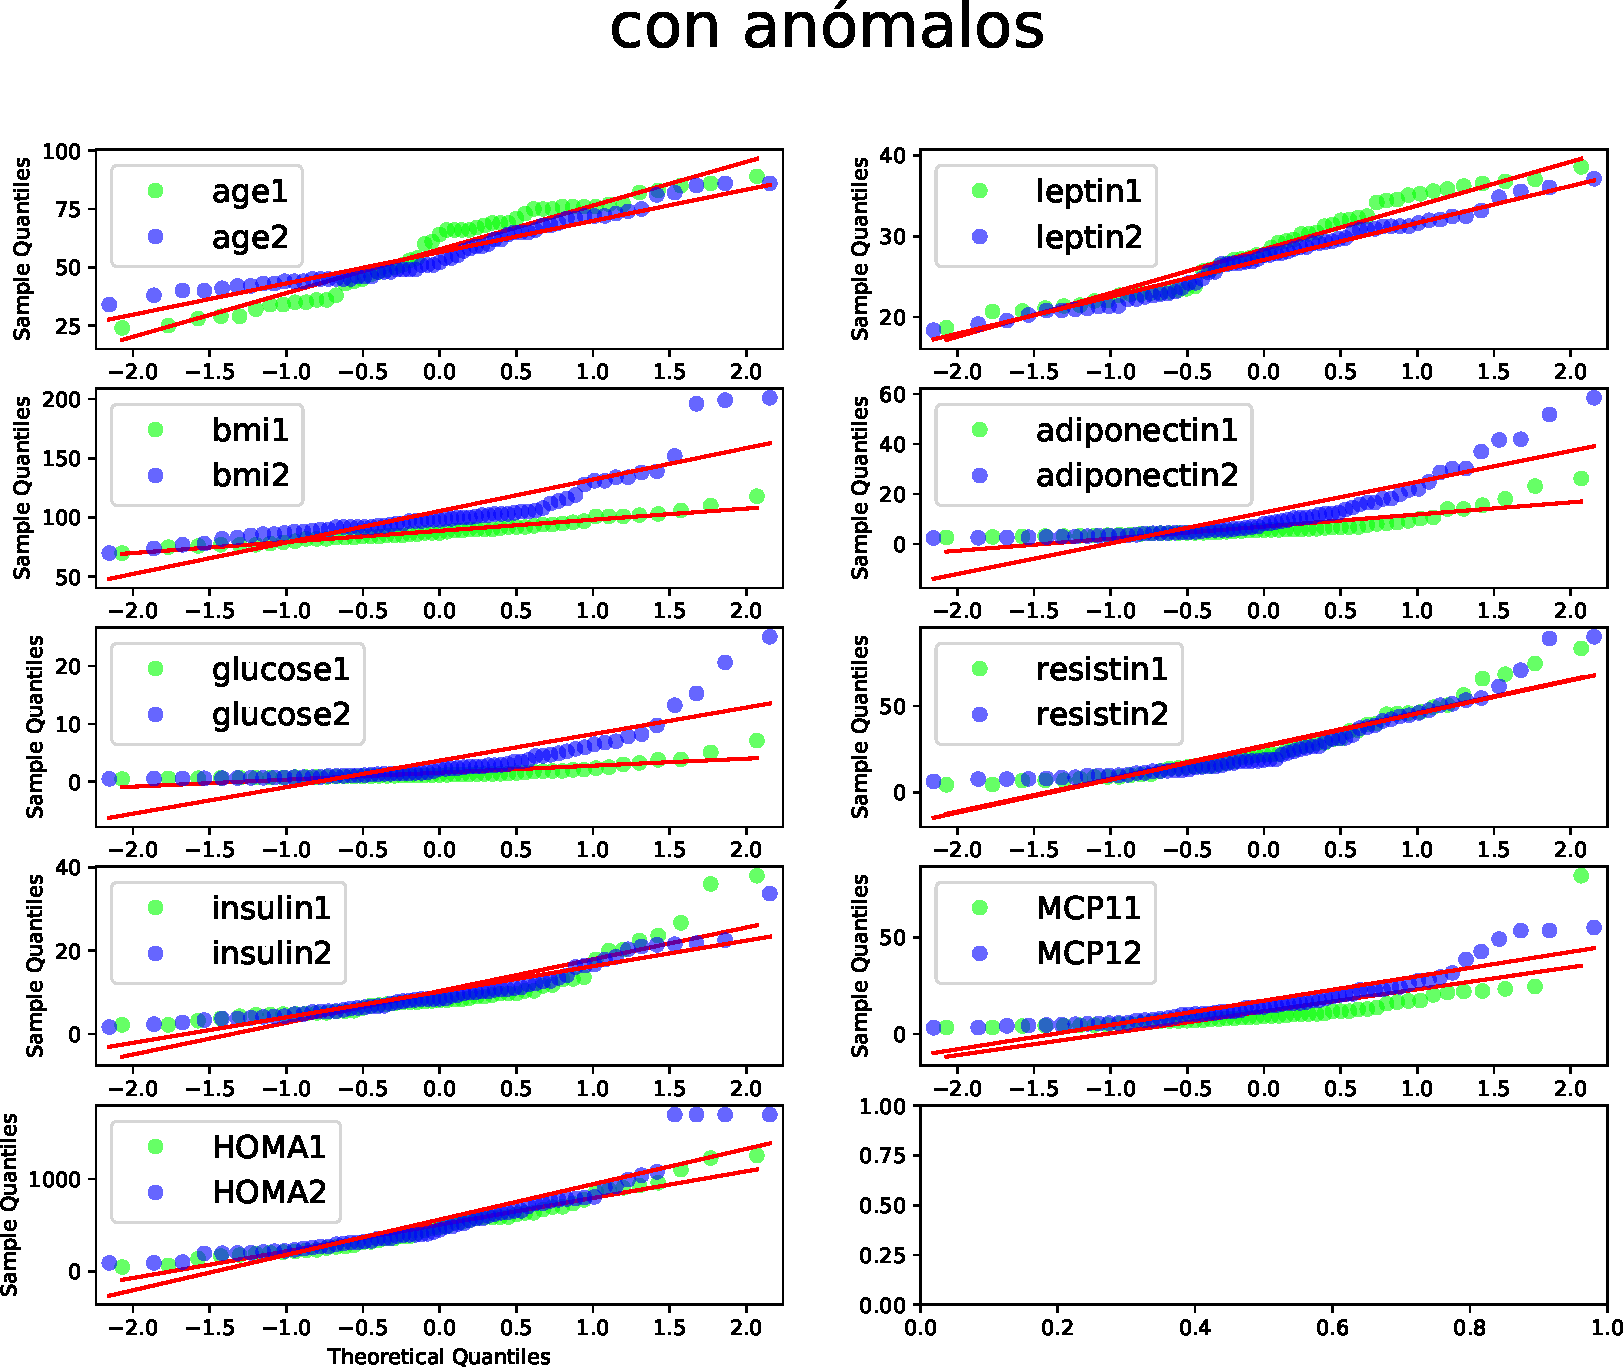
\includegraphics[width = 0.49\linewidth]{../python/images/qqp.pdf}
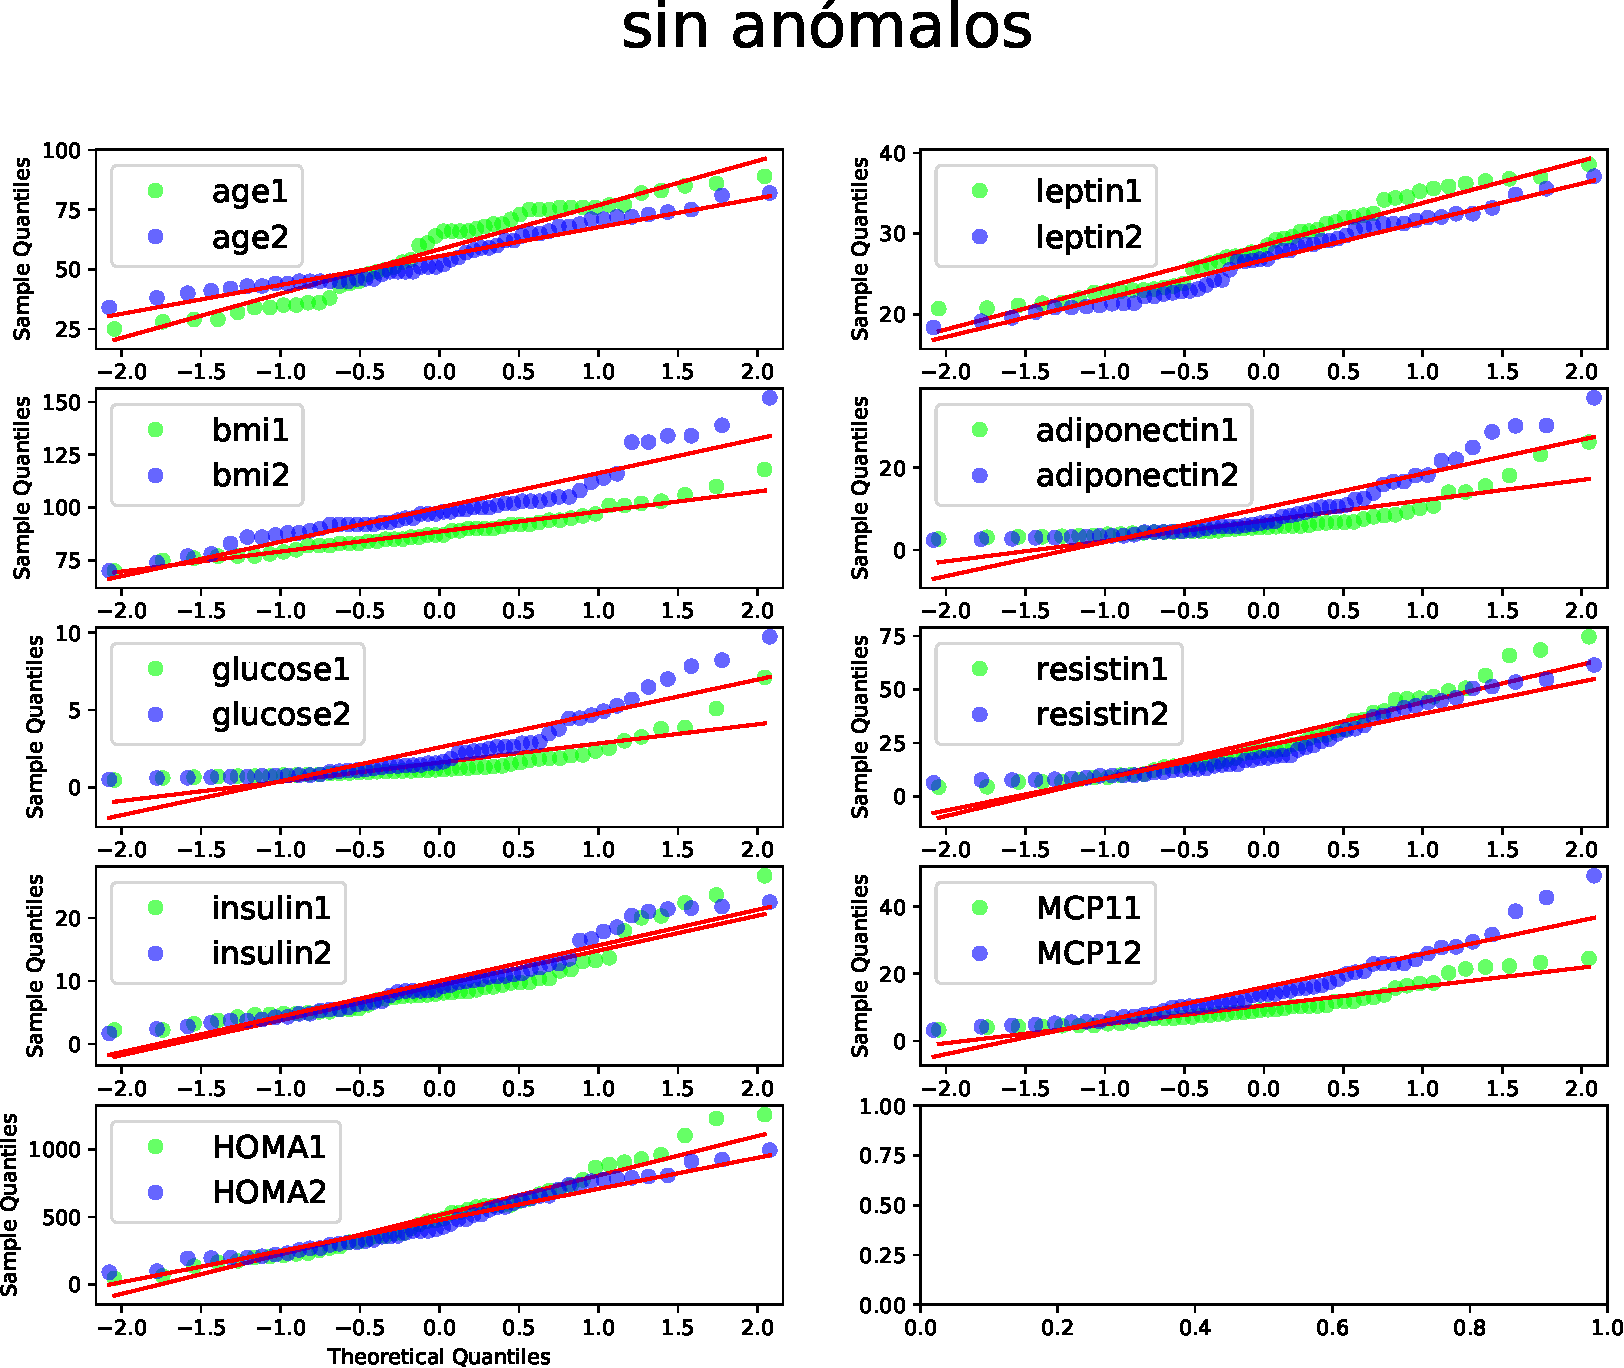
\includegraphics[width = 0.49\linewidth]{../python/images/qqp1.pdf}
\figcaption{QQplots Python para datos con y sin anomalias.}
\label{fig:qqps}
\end{figure}

\lstinputlisting[
	linerange = {9-28},
	caption = {[C\'odigo Python generador de los QQplots con datos an\'omalos.]
	\lstcaption{C\'odigo Python generador de los QQplots con datos an\'omalos.}},
	]{../python/src/qqplot.py}

\newpage
\begin{figure}[h]
\centering
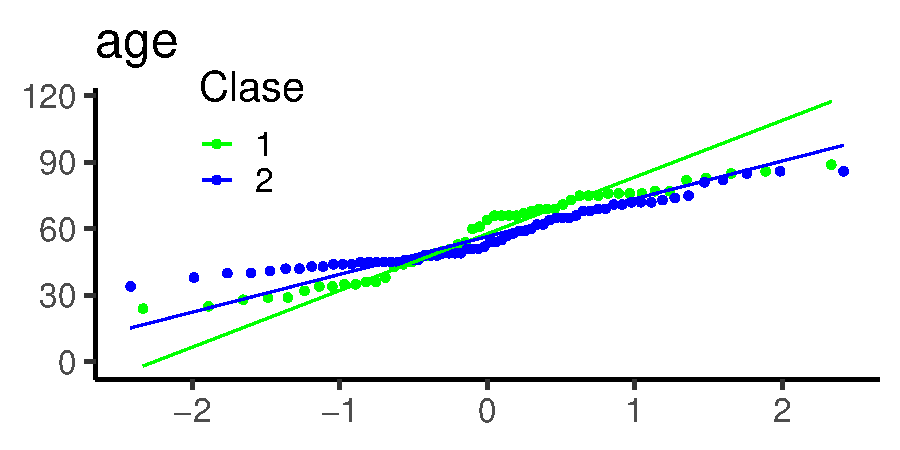
\includegraphics[width = 0.4\linewidth]{../R/images/qq1.pdf}
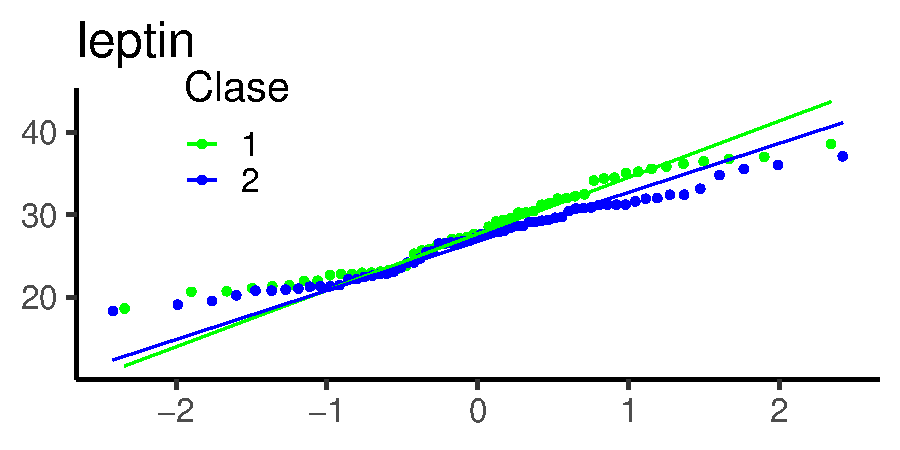
\includegraphics[width = 0.4\linewidth]{../R/images/qq2.pdf}
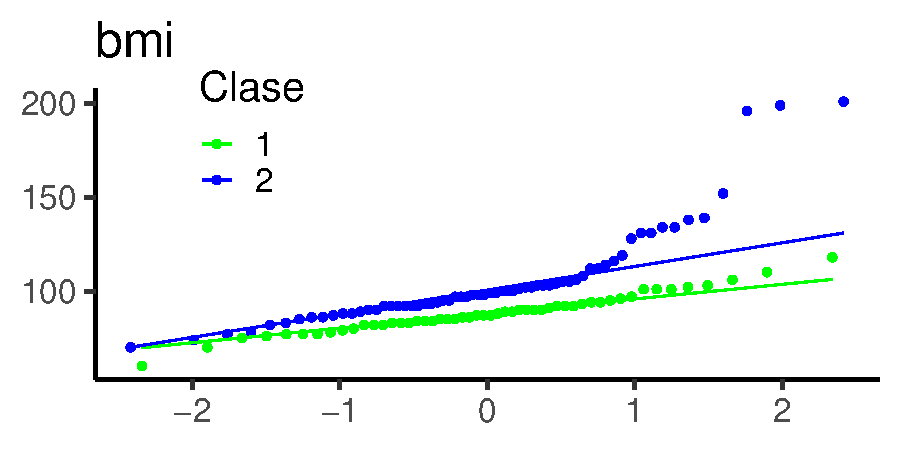
\includegraphics[width = 0.4\linewidth]{../R/images/qq3.pdf}
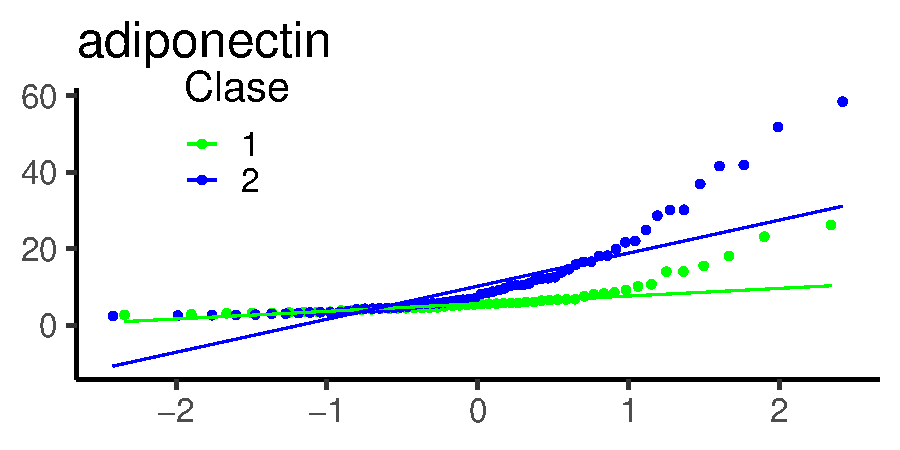
\includegraphics[width = 0.4\linewidth]{../R/images/qq4.pdf}
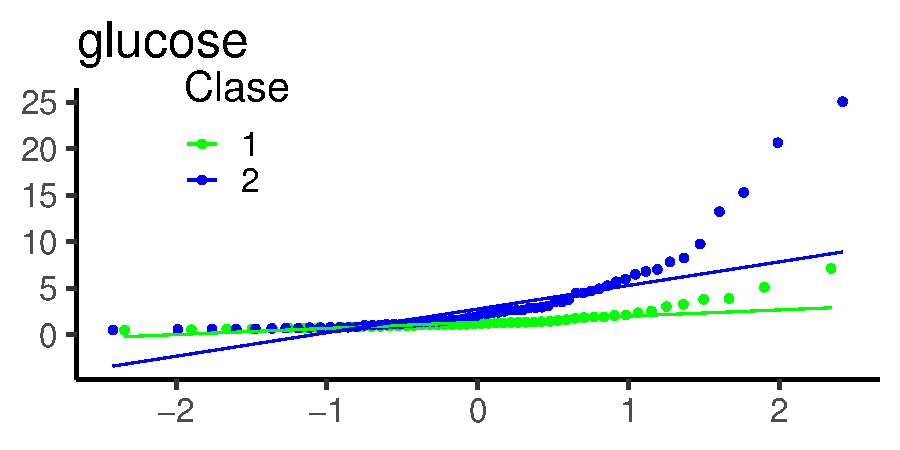
\includegraphics[width = 0.4\linewidth]{../R/images/qq5.pdf}
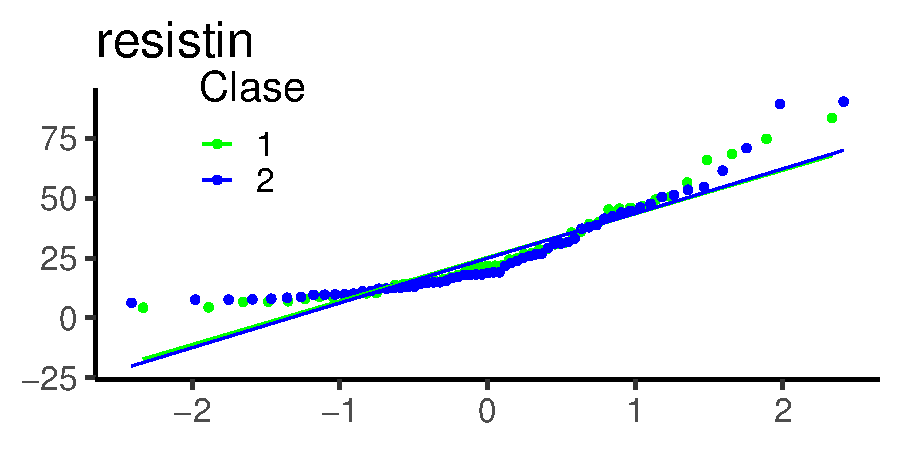
\includegraphics[width = 0.4\linewidth]{../R/images/qq6.pdf}
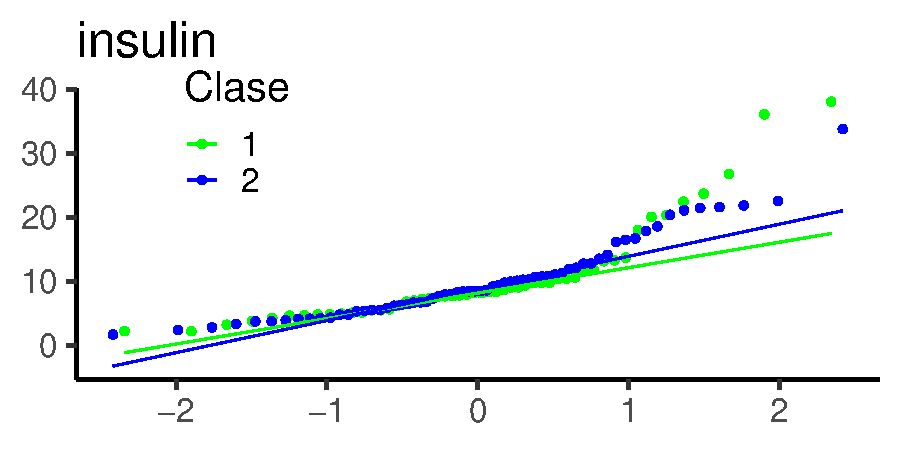
\includegraphics[width = 0.4\linewidth]{../R/images/qq7.pdf}
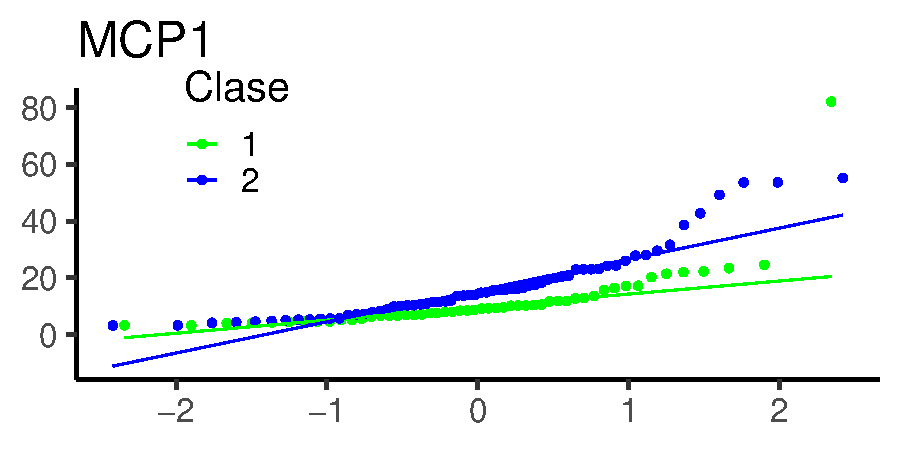
\includegraphics[width = 0.4\linewidth]{../R/images/qq8.pdf}
\includegraphics[width = 0.4\linewidth]{../R/images/qq9.pdf}
\includegraphics[width = 0.4\linewidth]{../R/images/qq10.pdf}
\figcaption{QQplots R.}
\label{fig:densR}
\end{figure}

\lstinputlisting[
	linerange = {8-18},
	caption = {[C\'odigo R generador de los QQplots.]
	\lstcaption{C\'odigo R generador de los QQplots.}},
	]{../R/src/qqplot.r}
\newpage

\begin{lstlisting}[
	style=Matlab-editor,
	frame=single,
	numbers=left,
	caption = {[C\'odigo Matlab generador de los QQplots.]
	\lstcaption{C\'odigo Matlab generador de los QQplots.}},
	captionpos=b,
	]
for (i = 1 : 10)
	subplot (5, 2, i);
	qqplot (dataR2mat (dataR2mat (:, end) == 1, i));
	hold on;
	qqplot (dataR2mat (dataR2mat (:, end) == 2, i));
end
\end{lstlisting}

\begin{figure}[h!]
\centering
\includegraphics[width = \linewidth]{../matlab/images/qqplo1.eps}
\figcaption{QQplots Matlab Clase 1.}
\end{figure}

\begin{figure}[h!]
\centering
\includegraphics[width = \linewidth]{../matlab/images/qqplo2.eps}
\figcaption{QQplots Matlab Clase 2.}
\end{figure}
\newpage

\subsubseccion{Corrplot}
\vfill
\begin{figure}[h]
\centering
\includegraphics[width = \linewidth]{../python/images/corrp.pdf}
\figcaption{Corrplot Python para datos con anomalias.}
\label{fig:cps}
\end{figure}
\vfill
\lstinputlisting[
	linerange = {13-18},
	caption = {[C\'odigo Python generador de los corrplots con datos an\'omalos.]
	\lstcaption{C\'odigo Python generador de los corrplots con datos an\'omalos.}},
	]{../python/src/corrplot.py}
\vfill

\newpage

\phantom{}
\vfill

\begin{figure}[h!]
\centering
\includegraphics[width = \linewidth]{../python/images/corrp1.pdf}
\figcaption{Corrplot Python para datos sin anomalias.}
\label{fig:cp1s}
\end{figure}

\vfill

\newpage
\begin{figure}[h]
\centering
\includegraphics[width = \linewidth]{../R/images/corrplot.pdf}
\figcaption{Corrplot R para datos con anomalias.}
\label{fig:corrR}
\end{figure}

\lstinputlisting[
	linerange = {9-18},
	caption = {[C\'odigo R generador de los corrplots.]
	\lstcaption{C\'odigo R generador de los corrplots.}},
	]{../R/src/corrplot.r}

\newpage
\begin{figure}[h]
\centering
\includegraphics[width = \linewidth]{../R/images/corrplot1.pdf}
\figcaption{Matriz de correlaciones en R.}
\label{fig:corrR1}
\end{figure}

\newpage
\begin{lstlisting}[
	style=Matlab-editor,
	frame=single,
	numbers=left,
	caption = {[C\'odigo Matlab generador de los corrplots.]
	\lstcaption{C\'odigo Matlab generador de los corrplots.}},
	captionpos=b,
	]
corrplot (dataR2mat (:,1:end-1))
\end{lstlisting}

\begin{figure}[h]
\centering
\includegraphics[width = \linewidth]{../matlab/images/corrplot1.eps}
\figcaption{Matriz de correlaciones en Matlab.}
\end{figure}
\newpage

\subseccion{Extracción de características.}

\subsubseccion{Filter Methods}

\lstinputlisting[
	linerange = {16 - 32},
	caption = {[M\'etodos filter Python.]
	\lstcaption{M\'etodos filter Python.}},
	]{../python/src/featureselection.py}

\begin{lstlisting}[
	caption = {[Ranking de variables seg\'un los m\'etodos filter Python.]
	{\lstcaption{Ranking de variables seg\'un los m\'etodos filter Python.}}},
	]
[4 5 9 6 7 3 1 8 2] -> fscore
[1 9 8 7 6 5 4 2 3] -> relieff
[3 4 1 1 1 2 3 6 1] -> diferencias
2.4444444444444446  -> media
\end{lstlisting}

\begin{lstlisting}[
	style=Matlab-editor,
	frame=single,
	numbers=left,
	caption = {[Ranking de variables Matlab.]
	{\lstcaption{Ranking de variables Matlab.}}},
	captionpos=b,
	]
[out   , rank]   = fscore  (x, y);
[RANKED, WEIGHT] = relieff (x, y, 1); % k = 1 neighbour 
diferencia = abs(rank-RANKED')
media = mean (diferencia) 
    var1  var2  var3  var4  var5  var6  var7  var8 var9
     3     5     4     8     2     9     1     6     7    -> fscore
     1     3     2     7     4     5     8     9     6    -> relieff
diferencias =
     2     2     2     1     2     4     7     3     1
media =
     2.6667 
\end{lstlisting}


\newpage
\begin{lstlisting}[
	caption =  {[Ranking de variables seg\'un distintos m\'etodos en R.]
	{\lstcaption{Ranking de variables seg\'un distintos m\'etodos en R.}}},
	]
# Fscore
library (PredPsych)
rank (fscore (datos, 10, 1:9))
#  age  leptin  bmi adiponectin  glucose  resistin  insulin MCP1  HOMA
#    3       5    9           7        8         2        1    6     4

# Relieff
brary (CORElearn)
rank (attrEval (as.factor (clase)~., datos, 'Relief'))
#  age  leptin  bmi adiponectin  glucose  resistin  insulin  MCP1  HOMA
#    9       7    8           2        4         5        1     6     3

# Algunos de los posibles metodos
for (i in infoCore (what = "attrEval")){
    cat (i, '\r\t\t', unname (rank (attrEval (as.factor (clase)~., datos, i))),'\n')
}
# ReliefFequalK    9 3 8 4 6 5 2 7 1
# ReliefFexpRank   8 5 9 3 6 4 1 7 2
# ReliefFbestK     9 7 8 3 4 5 1 6 2
# Relief           9 7 8 2 4 5 1 6 3
# InfGain          7 4 9 5 8 2 1 6 3
# GainRatio        9 2 8 7 6 4.5 1 3 4.5
# MDL              7 4 9 5 8 3 1 6 2
# Gini             7 4 9 5 8 3 1 6 2
# MyopicReliefF    6 4 9 5 7 3 1 8 2
# Accuracy         6 4 9 5 7 3 1.5 8 1.5
# ReliefFmerit     8 3 9 5 6 4 1 7 2
# ReliefFdistance  8 4 9 5 6 3 1 7 2
# ReliefFsqrDistan 8 4 9 5 6 3 1 7 2
# DKM              7 3 9 6 8 2 1 5 4
# ReliefFexpC      8 5 9 3 6 4 1 7 2
# ReliefFavgC      8 5 9 3 6 4 1 7 2
# ReliefFpe        8 5 9 3 6 4 1 7 2
# ReliefFpa        8 5 9 3 6 4 1 7 2
# ReliefFsmp       8 5 9 3 6 4 1 7 2
# GainRatioCost    9 2 8 7 6 4.5 1 3 4.5
# DKMcost          7 4 9 5 8 3 2 6 1
# 		.  .  .
\end{lstlisting}

\newpage
\subsubseccion{Wrapper Methods}

\lstinputlisting[
	linerange = {38 - 58},
	caption = {[Aplicaci\'on m\'etodos \textit{wrapper} de selecci\'on caracter\'isticas.]
	\lstcaption{Aplicaci\'on m\'etodos \textit{wrapper} de selecci\'on caracter\'isticas.}},
	]{../python/src/featureselection.py}

\begin{lstlisting}[
	caption = { [Resultados Python del filtrado mediante wrappers.]
	{\lstcaption{Resultados Python del filtrado mediante wrappers.}}},
	]
0.7054545454545454
Sequential Forward  Selection ('leptin', 'bmi', 'glucose', 'MCP1')

0.7094949494949495
Sequential Backward Selection ('leptin', 'bmi', 'glucose', 'insulin')
\end{lstlisting}
\newpage

\begin{lstlisting}[
	caption = {[Resultados R del filtrado mediante wrappers.]
	{\lstcaption{Resultados R del filtrado mediante wrappers.}}},
	]
# Sequential Feature Selector
library (mlr)
# Forward
sfs <- selectFeatures (
      learner    = makeLearner      ('classif.knn', k = 9, l = 3),
      task       = makeClassifTask  (data = datos, target = 'clase'),
      resampling = makeResampleDesc ("CV", iter = 50),
      control    = makeFeatSelControlSequential (method = "sfs", maxit = 100L))
# FeatSel result:
# Features (4): age, leptin, bmi, MCP1
# mmce.test.mean=0.1833333

# Backward
sbs <- selectFeatures (
      learner    = makeLearner      ('classif.knn', k = 9, l = 3),
      task       = makeClassifTask  (data = datos, target = 'clase'),
      resampling = makeResampleDesc ("CV", iter = 50),
      control    = makeFeatSelControlSequential (method = "sbs", maxit = 100L))
# FeatSel result:
# Features (4): age, leptin, bmi, MCP1
# mmce.test.mean=0.1800000
\end{lstlisting}

\vfill
\begin{lstlisting}[
	style=Matlab-editor,
	frame=single,
	numbers=left,
	caption = {[Resultados Matlab del filtrado mediante wrappers.]
	{\lstcaption{Resultados Matlab del filtrado mediante wrappers.}}},
	captionpos=b,
	]
fun = @(XT,yT,Xt,yt) ...
	      (sum ((yt - classify (Xt,XT,yT,'quadratic'))~=0));
fsf = sequentialfs (fun, x, y,'direction', 'forward', 'cv', 10);
fsb = sequentialfs (fun, x, y,'direction', 'backward', 'cv', 10);
[fsf' fsb']'
ans =
   1   0   0   0   0   0   0   0   0   -> forward
   1   1   1   1   0   0   1   1   0   -> backward
\end{lstlisting}
\vfill

% \begin{lstlisting}[
%         caption =   {[M\'etodo Boruta \textit{wrapper} de Random Forest R.]
%         {\lstcaption{M\'etodo Boruta \textit{wrapper} de Random Forest R.}}},
%         ]
% # esto es extra
% library (Boruta)
% Boruta (as.factor (clase)~., datos, maxRuns = 101) -> borutaout

% # Boruta performed 100 iterations in 4.317041 secs.
% #  5 attributes confirmed important: age, bmi, glucose, leptin, MCP1;
% #  3 attributes confirmed unimportant: HOMA, insulin, resistin;
% #  1 tentative attributes left: adiponectin;

% pdf ("../images/boruta.pdf")
% plot (borutaout, las = 2, xlab = '', main = 'Boruta Variable Importance')
% dev.off ()
% \end{lstlisting}

% \newpage
% \phantom{}
% \vfill
% \begin{figure}[h]
% \centering \includegraphics[width = 0.8\linewidth]{../R/images/boruta.pdf} \figcaption{Representación gráfica de la importancia de las variables
	% seleccionadas por Boruta.}
% \label{fig:bor}
% \end{figure}
% \vfill
% \phantom{}
\newpage
\subsubseccion{PCA}
\vspace{1cm}
\lstinputlisting[
	linerange = {60-65},
	caption = {[\textit{Principal Component Analysis} Python.]
	\lstcaption{\textit{Principal Component Analysis} Python.}},
	]{../python/src/featureselection.py}
\begin{lstlisting}[
	caption = {[Varianza explicada por componente y suma acumulada Python.]
       {\lstcaption{Varianza explicada por componente y suma acumulada Python.}}},
	]
[0.29146865 0.18490568 0.14125105 0.11727276 0.08486126 0.07999359
 0.06636991 0.03254865 0.00132847]
[0.29146865 0.47637432 0.61762537 0.73489813 0.81975939 0.89975298
0.96612289 0.99867153 1.        ]
\end{lstlisting}

\lstinputlisting[
	linerange = {7-8},
	caption = {[\textit{Principal Component Analysis} R.]
	\lstcaption{\textit{Principal Component Analysis} R.}},
	]{../R/src/pca.r}

\begin{lstlisting}[
	caption = {[Varianza explicada por componente y suma acumulada R.]
       {\lstcaption{Varianza explicada por componente y suma acumulada R.}}},
	]
Importance of components:
                PC1    PC2    PC3   PC4   PC5    PC6    PC7     PC8     PC9
Std deviation   1.7475 1.2393 1.082 1.048 0.8528 0.8144 0.66261 0.53101 0.17555
Propor. of Var. 0.3393 0.1707 0.130 0.122 0.0808 0.0737 0.04878 0.03133 0.00342
Cum. Var.       0.3393 0.5100 0.640 0.762 0.8428 0.9165 0.96525 0.99658 1.00000
\end{lstlisting}

\begin{lstlisting}[
	style=Matlab-editor,
	frame=single,
	numbers=left,
	caption = {[\textit{Principal Component Analysis} Matlab y pareto.]
	\lstcaption{\textit{Principal Component Analysis} Matlab y pareto.}},
	captionpos=b,
	]
x = zscore (x);
[coeff, score, latent] = pca (x);
pareto (latent)
\end{lstlisting}

\newpage

\subsubseccion{Pareto}
\vspace{0.9cm}
\lstinputlisting[
	linerange = {93-100},
	caption = {[C\'odigo generador del diagrama de Pareto en Python.]
	\lstcaption{C\'odigo generador del diagrama de Pareto en Python.}},
	]{../python/src/featureselection.py}

\lstinputlisting[
	linerange = {12-32},
	caption = {[C\'odigo generador del diagrama de Pareto en R.]
	\lstcaption{C\'odigo generador del diagrama de Pareto en R.}},
	]{../R/src/pca.r}


\newpage
\phantom{}
\vfill{}
\begin{figure}[h]
\centering
\includegraphics[width = 0.49\linewidth]{../python/images/pareto.pdf}
\includegraphics[width = 0.49\linewidth]{../R/images/pareto.pdf}
	\figcaption{Diagrama de Pareto en Python y R.}
\label{fig:pareto}
\end{figure}

\vspace{0.9cm}

\begin{figure}[h]
\centering
\includegraphics[width = 0.49\linewidth]{../matlab/images/pareto.eps}
	\figcaption{Diagrama de Pareto en Matlab.}
\label{fig:pareto}
\end{figure}
\vfill{}
\newpage
\subsubseccion{Biplot}

\begin{figure}[h]
\centering
\includegraphics[width = 0.7\linewidth]{../python/images/biplotpca.pdf}
\figcaption{Biplot Python.}
\label{fig:biplotP}
\end{figure}

\lstinputlisting[
	linerange = {71-89},
	caption = {[C\'odigo generador del Biplot en Python.]
	\lstcaption{C\'odigo generador del Biplot en Python.}},
	]{../python/src/featureselection.py}

\newpage
\begin{figure}[h]
\centering
\includegraphics[width = 0.8\linewidth]{../R/images/biplot.pdf}
\figcaption{Biplot R.}
\label{fig:biplotR}
\end{figure}
\lstinputlisting[
	linerange = {34-48},
	caption = {[C\'odigo generador del Biplot en R.]
	\lstcaption{C\'odigo generador del Biplot en R.}},
	]{../R/src/pca.r}
\newpage
\seccion{Modelos de Clasificación}

\subseccion{Clasificación Lineal}
\vfill
\lstinputlisting[
	linerange = {19-36},
	caption = {[Python validaci\'on del modelo lineal.]
	\lstcaption{Python validaci\'on del modelo lineal.}},
	]{../python/src/clasificadorlineal1.py}
\vfill
\begin{lstlisting}[
	caption = {[Python validaci\'on seg\'un distintos m\'etodos de partici\'on.]
       {\lstcaption{Python validaci\'on seg\'un distintos m\'etodos de partici\'on.}}},
	]
Linear puntuacion CV media: 0.75 std: 0.13
Linear puntuacion KF media: 0.75 std: 0.10
Linear puntuacion SS media: 0.71 std: 0.14
Linear puntuacion LO media: 0.76 std: 0.43
\end{lstlisting}
\vfill

\newpage

\phantom{}
\vfill
\lstinputlisting[
	linerange = {14-37},
	mathescape=false,
	caption = {[R an\'alisis lineal discriminante.]
	\lstcaption{R an\'alisis lineal discriminante.}},
	]{../R/src/clasificacion.r}
\vfill
\begin{lstlisting}[
	caption = {[R puntuaci\'on de mil evaluaciones.]
       {\lstcaption{R puntuaci\'on de mil evaluaciones.}}},
	]
	  vars   n  mean   sd median trimmed  mad  min  max range  skew
ldascores    1 1000 0.72 0.08   0.73    0.72 0.10 0.47 0.97  0.50 -0.09
\end{lstlisting}
\vfill

\newpage
\subseccion{Clasificación Cuadrática}
\vfill
\lstinputlisting[
	linerange = {40-58},
	caption = {[Python validaci\'on del modelo cuadr\'atico.]
	\lstcaption{Python validaci\'on del modelo cuadr\'atico.}},
	]{../python/src/clasificadorlineal1.py}
\vfill
\begin{lstlisting}[
	caption = {[Python validaci\'on seg\'un distintos m\'etodos de partici\'on.]
       {\lstcaption{Python validaci\'on seg\'un distintos m\'etodos de partici\'on.}}},
	]
Quadratic puntuacion CV media: 0.66 std: 0.19
Quadratic puntuacion KF media: 0.76 std: 0.09
Quadratic puntuacion SS media: 0.76 std: 0.14
Quadratic puntuacion LO media: 0.73 std: 0.44
\end{lstlisting}
\vfill
\newpage
\phantom{}
\vfill
\lstinputlisting[
	linerange = {42-63},
	mathescape=false,
	caption = {[R an\'alisis cuadr\'atico discriminante.]
	\lstcaption{R an\'alisis cuadr\'atico discriminante.}},
	]{../R/src/clasificacion.r}
\vfill
\begin{lstlisting}[
	caption = {[R puntuaci\'on de mil evaluaciones.]
       {\lstcaption{R puntuaci\'on de mil evaluaciones.}}},
	]
     vars        n mean   sd median trimmed  mad  min  max range  skew
qdascores    2 1000 0.69 0.07   0.70    0.69 0.10 0.43 0.87  0.43 -0.17
\end{lstlisting}
\vfill

\newpage
\subseccion{Clasificación KNN}
\vfill

\lstinputlisting[
	linerange = {15-33},
	caption = {[Python validaci\'on del modelo KNN.]
	\lstcaption{Python validaci\'on del modelo KNN.}},
	]{../python/src/clasificadorknn.py}

\vfill
\begin{lstlisting}[
	caption = {[Python validaci\'on seg\'un distintos m\'etodos de partici\'on.]
       {\lstcaption{Python validaci\'on seg\'un distintos m\'etodos de partici\'on.}}},
	]
KNN puntuacion CV media: 0.47 std: 0.12
KNN puntuacion KF media: 0.47 std: 0.15
KNN puntuacion SS media: 0.47 std: 0.13
KNN puntuacion LO media: 0.43 std: 0.50
\end{lstlisting}
\vfill

\newpage
\phantom{}
\vfill
\lstinputlisting[
	linerange = {66-89},
	mathescape=false,
	caption = {[R \textit{K nearest neighbours}.]
	\lstcaption{R \textit{K nearest neighbours}.}},
	]{../R/src/clasificacion.r}
\vfill
\begin{lstlisting}[
	caption = {[R puntuaci\'on de mil evaluaciones.]
       {\lstcaption{R puntuaci\'on de mil evaluaciones.}}},
	]
     vars        n mean   sd median trimmed  mad  min  max range  skew
knnscores    3 1000 0.66 0.07   0.67    0.66 0.05 0.43 0.90  0.47 -0.07
\end{lstlisting}
\vfill
\newpage
\seccion{Postámbulo}

\subseccion{Comparación \textit{LDA}, \textit{QDA}, \textit{KNN} R.}
\vfill
\begin{figure}[h!]
\centering
\includegraphics[width = 0.9\linewidth]{../R/images/scores.pdf}
\figcaption{Comparación de mil evaluaciones de cada uno de los métodos de clasificación en R.}
\end{figure}
\vfill
\newpage

\subseccion{Puntuación \textit{knn} vs. número de vecinos.}
\begin{figure}[h!]
\centering
\includegraphics[width = 0.7\linewidth]{../python/images/knn.pdf}
\figcaption{Rendimineto decreciente según aumenta el número de vecinos.}
\label{fig:knn}
\end{figure}

\lstinputlisting[
	linerange = {37-55},
	caption = {[Evoluci\'on de puntuaci\'on seg\'un n\'umero de vecinos.]
	\lstcaption{Evoluci\'on de puntuaci\'on seg\'un n\'umero de vecinos.}},
	]{../python/src/clasificadorknn.py}

\newpage
\subseccion{\textit{Benchmarking}}
\lstinputlisting[
	linerange = {10-46},
	mathescape=false,
	caption = {[C\'odigo R para evaluar el tiempo de ejecucci\'on.]
	\lstcaption{C\'odigo R para evaluar el tiempo de ejecucci\'on.}},
	]{../R/src/benchmarking.r}
\newpage
\lstinputlisting[
	linerange = {12-43, 61-63},
	mathescape=false,
	caption = {[C\'odigo Python para evaluar el tiempo de ejecucci\'on.]
	\lstcaption{C\'odigo Python para evaluar el tiempo de ejecucci\'on.}},
	]{../python/src/benchmarking.py}

\newpage
\begin{lstlisting}[
	caption = {[Tiempo de ejecuci\'on en R.]
       {\lstcaption{Tiempo de ejecuci\'on en R.}}},
	]
    test replications elapsed relative user.self sys.self
1  1 load        1000   4.803    8.486     4.712    0.090
2  2 part        1000  13.267   23.440    13.201    0.061
3  3 lda         1000   3.359    5.935     3.346    0.013
4  4 qda         1000   3.480    6.148     3.455    0.025
5  5 knn         1000   0.566    1.000     0.562    0.004
\end{lstlisting}

\begin{lstlisting}[
	caption = {[Tiempo de ejecuci\'on en Python.]
       {\lstcaption{Tiempo de ejecuci\'on en Python.}}},
	]
'loa' ((), {}) 0.00376701354980468750 sec
'par' ((), {}) 0.00057792663574218750 sec
'lda' ((), {}) 0.00213122367858886719 sec
'qda' ((), {}) 0.00131011009216308594 sec
'lda' ((), {}) 0.00145196914672851562 sec
Result: qda is 1.516303298299778 times faster than lda
Result: qda is 2.87883278273268 times faster than knn
Result: lda is 1.918905609112522 times faster than knn
\end{lstlisting}

\begin{lstlisting}[
	caption = {[Caracter\'isticas de la m\'aquina usada.]
       {\lstcaption{Caracter\'isticas de la m\'aquina usada.}}},
	]
OS: macOS Sierra 10.12.6 16G1618 x86_64
Host: iMac12,2
Kernel: 16.7.0
Uptime: 4d 23h
Packages: 292 (port), 233 (brew)
Shell: zsh 5.2
Resolution: 2560x1440
DE: Aqua
WM: Kwm
Terminal: kitty
CPU: Intel i5-2500S (4) @ 2.70GHz
GPU: AMD Radeon HD 6770M
Memory: 7027MiB / 12288MiB
Disk (/): 806G / 931G (87%)
\end{lstlisting}

\newpage
\subseccion{Curva ROC}

\begin{figure}[h]
\centering
\includegraphics[width = 0.8\linewidth]{../R/images/roc.pdf}
\figcaption{ROC R.}
\label{fig:roc}
\end{figure}

\lstinputlisting[
	linerange = {37-47},
	mathescape=false,
	caption = {[C\'odigo R para generar la curva ROC y la AUC.]
	\lstcaption{C\'odigo R para generar la curva ROC y la AUC.}},
	]{../R/src/roc.r}

\end{document}
